\chapter{Sprint 1 : Fondation \& Gestion des Ressources}

\section*{Introduction}
\addcontentsline{toc}{section}{Introduction}
Le Sprint~1 constitue la fondation technique de Fleet~AI. Il met en place les mécanismes d'authentification unifiée via la passerelle WFMS et le contrôle d'accès par rôles, garantissant que chaque acteur n'accède qu'aux fonctionnalités qui lui sont attribuées. Les référentiels opérationnels — utilisateurs, véhicules, chauffeurs et zones géographiques — sont créés et gérés depuis l'interface web. Le journal d'audit et les sauvegardes assurent la traçabilité et la sécurité des données. En parallèle, l'application mobile Flutter est initialisée pour les Chauffeurs, leur permettant de se connecter, de consulter leurs indicateurs de performance et de déclarer leur disponibilité. Ce premier sprint pose les bases sur lesquelles tous les sprints suivants vont s'appuyer.

\clearpage

\section{Sprint Backlog}

\textbf{Objectif du sprint :} L'objectif est de mettre en place l'authentification WFMS, le contrôle d'accès par rôles et les référentiels de base — utilisateurs, véhicules, chauffeurs, zones — ainsi que le journal d'audit, les sauvegardes et l'application mobile Chauffeur.

\definecolor{headerbg}{HTML}{d5f5e3}
\setlength{\arrayrulewidth}{1pt}

Les story points (SP) sont estimés par l'équipe de développement selon la suite de Fibonacci (1, 2, 3, 5, 8, 13, \ldots). Chaque valeur reflète la \textbf{complexité fonctionnelle}, l'\textbf{effort} et le \textbf{risque} associé à la User Story, et non une durée en heures. L'échelle retenue est : 1--2 (tâche simple, déjà maîtrisée), 3--5 (complexité modérée), 8--13 (tâche complexe ou comportant une forte incertitude).

\begin{longtable}{|>{\raggedright\arraybackslash}p{4.2cm}|>{\raggedright\arraybackslash}p{4.8cm}|>{\raggedright\arraybackslash}p{4.5cm}|c|}
\hline
\rowcolor{headerbg}
\textbf{User Story} & \textbf{Tâche} & \textbf{Critères d'acceptation} & \textbf{\rotatebox{90}{SP}} \\
\hline
\endfirsthead
\hline
\rowcolor{headerbg}
\textbf{User Story} & \textbf{Tâche} & \textbf{Critères d'acceptation} & \textbf{\rotatebox{90}{SP}} \\
\hline
\endhead
\hline
\endfoot

%------ US-001 ------
\multirow{2}{=}{En tant qu'utilisateur, je veux me connecter avec mes identifiants habituels afin d'accéder aux fonctionnalités Fleet~AI correspondant à mon rôle.}
& Mettre en place la vérification des identifiants à la connexion afin de valider l'accès de l'utilisateur. & L'utilisateur peut se connecter avec ses identifiants habituels ; un message clair s'affiche en cas d'erreur. & 3 \\
\cline{2-4}
& Rediriger chaque utilisateur vers son espace dédié selon son rôle après connexion réussie. & Chaque rôle accède à son interface dédiée après authentification. & 2 \\
\hline

%------ US-002 ------
\multirow{2}{=}{En tant qu'Administrateur, je veux que les droits de chaque utilisateur soient contrôlés à chaque accès afin que chacun n'utilise que les fonctionnalités autorisées par son rôle.}
& Contrôler les droits d'accès de l'utilisateur à chaque action sensible selon son rôle. & Un utilisateur sans les droits requis se voit refuser l'accès avec un message explicite ; son rôle détermine ses permissions. & 3 \\
\cline{2-4}
& Valider que chaque rôle accède uniquement aux fonctionnalités qui lui sont autorisées. & Les accès autorisés et refusés sont cohérents avec les droits définis par rôle pour tous les profils du système. & 2 \\
\hline

%------ US-003 ------
\multirow{2}{=}{En tant qu'Administrateur, je veux gérer les comptes utilisateurs afin de contrôler les accès au système.}
& Permettre à l'Administrateur de créer, modifier et désactiver des comptes utilisateurs selon leur rôle. & Le CRUD complet fonctionne ; un compte désactivé ne peut plus accéder au système. & 3 \\
\cline{2-4}
& Mettre à disposition de l'Administrateur une interface de gestion des comptes avec liste paginée et formulaires. & La liste des utilisateurs est consultable avec filtres ; les formulaires de création et d'édition sont fonctionnels. & 2 \\
\hline

%------ US-004 ------
\multirow{2}{=}{En tant qu'Administrateur, je veux assigner un rôle à chaque utilisateur afin de définir ses permissions.}
& Associer un rôle unique à chaque utilisateur lors de sa création afin de définir ses droits dans le système. & Le rôle attribué détermine les fonctionnalités accessibles ; les permissions sont vérifiées à chaque action. & 3 \\
\cline{2-4}
& Présenter la liste des rôles disponibles dans le formulaire de création d'utilisateur avec sélection obligatoire. & La liste des rôles est affichée ; la sélection est obligatoire avant validation du formulaire. & 2 \\
\hline

%------ US-005 ------
\multirow{2}{=}{En tant qu'Administrateur, je veux gérer les zones géographiques de livraison afin de structurer les opérations par région.}
& Permettre la création et la modification de zones géographiques définies par des polygones sur carte. & Les zones sont définies par polygone sur carte ; leur surface et périmètre sont calculés automatiquement. & 3 \\
\cline{2-4}
& Mettre à disposition une carte interactive permettant à l'Administrateur de dessiner et modifier les zones. & La carte interactive permet la création et l'édition des polygones de zones géographiques. & 2 \\
\hline

%------ US-006 ------
\multirow{2}{=}{En tant qu'Administrateur, je veux consulter le journal d'audit du système afin de tracer toutes les actions critiques.}
& Enregistrer automatiquement toutes les actions critiques (entité concernée, acteur, date, type d'action). & Les entrées du journal sont enregistrées pour chaque action ; filtrables par date, utilisateur, action et entité. & 3 \\
\cline{2-4}
& Mettre à disposition de l'Administrateur une interface de consultation du journal avec pagination et filtres. & La liste des entrées est paginée ; les filtres combinés fonctionnent correctement. & 2 \\
\hline

%------ US-007 ------
\multirow{2}{=}{En tant qu'Administrateur, je veux déclencher des sauvegardes des données afin de protéger les informations du système.}
& Permettre à l'Administrateur de déclencher une sauvegarde complète de la base de données. & La sauvegarde est effectuée et archivée avec horodatage ; l'Administrateur peut confirmer son succès. & 2 \\
\cline{2-4}
& Afficher à l'Administrateur l'historique des sauvegardes avec leur statut. & L'historique des sauvegardes est consultable avec statut mis à jour (en cours, terminée, échouée). & 1 \\
\hline

%------ US-008 ------
\multirow{2}{=}{En tant qu'Administrateur, je veux consulter le tableau de bord avec les statistiques générales afin de superviser l'état du système.}
& Calculer et exposer les indicateurs clés du système (utilisateurs actifs, véhicules, chauffeurs, zones, coûts). & Les indicateurs affichés sont corrects et filtrables par période. & 3 \\
\cline{2-4}
& Présenter les indicateurs et tendances sous forme de graphiques et de tableau de bord visuel. & Le tableau de bord affiche les KPIs, les tendances de coûts et l'activité récente. & 2 \\
\hline

%------ US-009 ------
\multirow{2}{=}{En tant que Planificateur, je veux consulter la liste des véhicules avec leur statut afin de connaître les ressources disponibles.}
& Mettre à disposition du Planificateur la liste des véhicules filtrée par statut et par zone. & La liste affiche le statut, la capacité (poids/volume), le kilométrage et la zone ; pagination intégrée. & 2 \\
\cline{2-4}
& Permettre au Planificateur de filtrer et trier la liste des véhicules selon ses besoins. & La liste des véhicules s'affiche avec filtres fonctionnels par statut et par zone. & 1 \\
\hline

%------ US-010 ------
\multirow{2}{=}{En tant qu'Administrateur, je veux gérer les véhicules afin de maintenir le référentiel à jour.}
& Permettre à l'Administrateur de créer, modifier et supprimer des véhicules, avec protection contre la suppression d'un véhicule en mission. & Un véhicule en mission ne peut être supprimé ; la suppression est logique et réversible. & 2 \\
\cline{2-4}
& Mettre à disposition de l'Administrateur un formulaire de création et modification des véhicules avec validation des champs. & Le formulaire valide tous les champs obligatoires ; la liste se met à jour après sauvegarde. & 1 \\
\hline

%------ US-011 ------
\multirow{2}{=}{En tant que Planificateur, je veux marquer un véhicule en maintenance afin de le retirer temporairement de la planification.}
& Permettre au Planificateur de changer le statut d'un véhicule vers « En maintenance », avec enregistrement dans le journal d'audit. & Le changement est immédiat ; le véhicule en maintenance est exclu des affectations. & 2 \\
\cline{2-4}
& Afficher une demande de confirmation au Planificateur avant le changement de statut du véhicule. & La confirmation est demandée avant l'action ; le statut est mis à jour dans la liste. & 1 \\
\hline

%------ US-012 ------
\multirow{2}{=}{En tant que Manager, je veux consulter le taux d'utilisation des véhicules afin d'optimiser la flotte.}
& Calculer le taux d'utilisation des véhicules à partir de leur historique de kilométrage. & Le taux est calculé par véhicule et de manière globale sur la période sélectionnée. & 3 \\
\cline{2-4}
& Présenter le taux d'utilisation sous forme de graphique par véhicule avec sélection de période. & Le graphique s'affiche par véhicule avec sélection de la période. & 2 \\
\hline

%------ US-013 ------
\multirow{2}{=}{En tant que Manager, je veux consulter les coûts par véhicule afin de suivre les dépenses opérationnelles.}
& Calculer et exposer les coûts par véhicule ventilés par catégorie (carburant, entretien, assurance). & Les coûts sont ventilés par catégorie ; les tendances mensuelles sont calculées. & 3 \\
\cline{2-4}
& Présenter les coûts sous forme de graphique et identifier les 5 véhicules les plus coûteux. & Le tableau de bord affiche les 5 véhicules les plus coûteux avec graphique mensuel. & 2 \\
\hline

%------ US-014 ------
\multirow{2}{=}{En tant que Planificateur, je veux consulter la disponibilité des chauffeurs afin de planifier les affectations.}
& Mettre à disposition du Planificateur un calendrier de disponibilité des chauffeurs avec filtres par type et par zone. & Le calendrier affiche les disponibilités par type (disponible, congé, mission) et par zone. & 3 \\
\cline{2-4}
& Permettre au Planificateur de filtrer les disponibilités par plage de dates et par zone. & La vue calendrier filtrée par date et par zone fonctionne correctement. & 2 \\
\hline

%------ US-015 ------
\multirow{2}{=}{En tant que Planificateur, je veux consulter les performances des chauffeurs afin de guider les affectations.}
& Calculer les indicateurs de performance des chauffeurs (taux de livraison, ponctualité, notation moyenne) selon les coefficients configurés. & Les indicateurs sont calculés selon les coefficients définis par l'Administrateur et affichés dans la fiche du chauffeur. & 3 \\
\cline{2-4}
& Présenter les indicateurs de performance du chauffeur avec des repères visuels dans son profil. & La fiche chauffeur affiche les indicateurs avec des repères visuels de niveau. & 2 \\
\hline

%------ US-016 ------
\multirow{2}{=}{En tant que Manager, je veux consulter le classement des chauffeurs afin d'identifier les plus et les moins performants.}
& Calculer et présenter le classement des chauffeurs selon leur score global pondéré. & Le classement est trié par score global ; accessible depuis le tableau de bord. & 2 \\
\cline{2-4}
& Afficher le classement des chauffeurs avec des indicateurs permettant d'identifier les plus et moins performants. & Le classement s'affiche avec indicateurs colorés de performance. & 1 \\
\hline

%------ US-017 ------
\multirow{2}{=}{En tant qu'Administrateur, je veux configurer les indicateurs de performance des chauffeurs afin d'adapter le calcul du score global.}
& Permettre à l'Administrateur de modifier les 3 coefficients de performance des chauffeurs ; toute modification est enregistrée dans le journal d'audit. & Les modifications sont tracées dans le journal d'audit. & 2 \\
\cline{2-4}
& Présenter un formulaire de configuration des coefficients avec validation de leur cohérence. & Le formulaire vérifie que les coefficients sont cohérents et la somme correcte avant enregistrement. & 1 \\
\hline

%------ US-018 ------
\multirow{2}{=}{En tant que Chauffeur, je veux me connecter à l'application mobile afin d'accéder à mes fonctionnalités Fleet~AI.}
& Permettre au Chauffeur de se connecter à l'application mobile avec ses identifiants habituels et de rester authentifié. & La connexion mobile fonctionne ; l'application Fleet~AI est accessible depuis l'application après authentification. & 3 \\
\cline{2-4}
& Permettre au Chauffeur d'accéder à l'application Fleet~AI depuis le menu de navigation de l'application mobile. & L'application Fleet~AI est accessible depuis le menu de navigation après connexion. & 2 \\
\hline

%------ US-019 ------
\multirow{2}{=}{En tant que Chauffeur, je veux consulter mes indicateurs de performance depuis l'application mobile afin de suivre mon activité.}
& Présenter au Chauffeur ses indicateurs de performance personnels sur l'application mobile. & L'écran affiche les indicateurs avec graphiques ; les coefficients de pondération sont ceux configurés par l'Administrateur. & 3 \\
\cline{2-4}
& Afficher les graphiques de performance sur l'application mobile de manière lisible. & Les graphiques de performance s'affichent correctement sur l'application mobile. & 2 \\
\hline

%------ US-020 ------
\multirow{2}{=}{En tant que Chauffeur, je veux déclarer ma disponibilité depuis l'application mobile afin de signaler mes périodes de présence et d'absence.}
& Permettre au Chauffeur de déclarer ses périodes de disponibilité ou d'absence depuis l'application mobile (types : disponible, congé, formation, mission). & La déclaration est enregistrée ; les chevauchements de créneaux sont détectés et signalés. & 3 \\
\cline{2-4}
& Valider les règles de disponibilité selon le type de contrat du chauffeur (officiel ou prestataire). & Les chauffeurs officiels ne peuvent déclarer que des absences ; les prestataires peuvent déclarer leur disponibilité. & 2 \\
\hline

%------ US-113/114 ------
\multirow{2}{=}{En tant qu'utilisateur, je veux configurer mes préférences de notifications et consulter mon historique depuis mon application.}
& Permettre à l'utilisateur de choisir ses canaux de notification (dans l'application, par email) par type d'événement. & L'utilisateur peut choisir les canaux par type d'événement et sauvegarder ses préférences. & 2 \\
\cline{2-4}
& Permettre à l'utilisateur de consulter l'historique de ses notifications depuis l'application web ou mobile. & Les préférences sont sauvegardées ; l'historique des notifications est accessible. & 1 \\
\hline

\caption{Sprint Backlog du Sprint 1 --- Fondation \& Gestion des Ressources (20 stories, 76 SP)}
\end{longtable}
\setlength{\arrayrulewidth}{0.4pt}


\section{Conception}

\subsection{Diagramme de cas d'utilisation}

\begin{figure}[H]
\centering
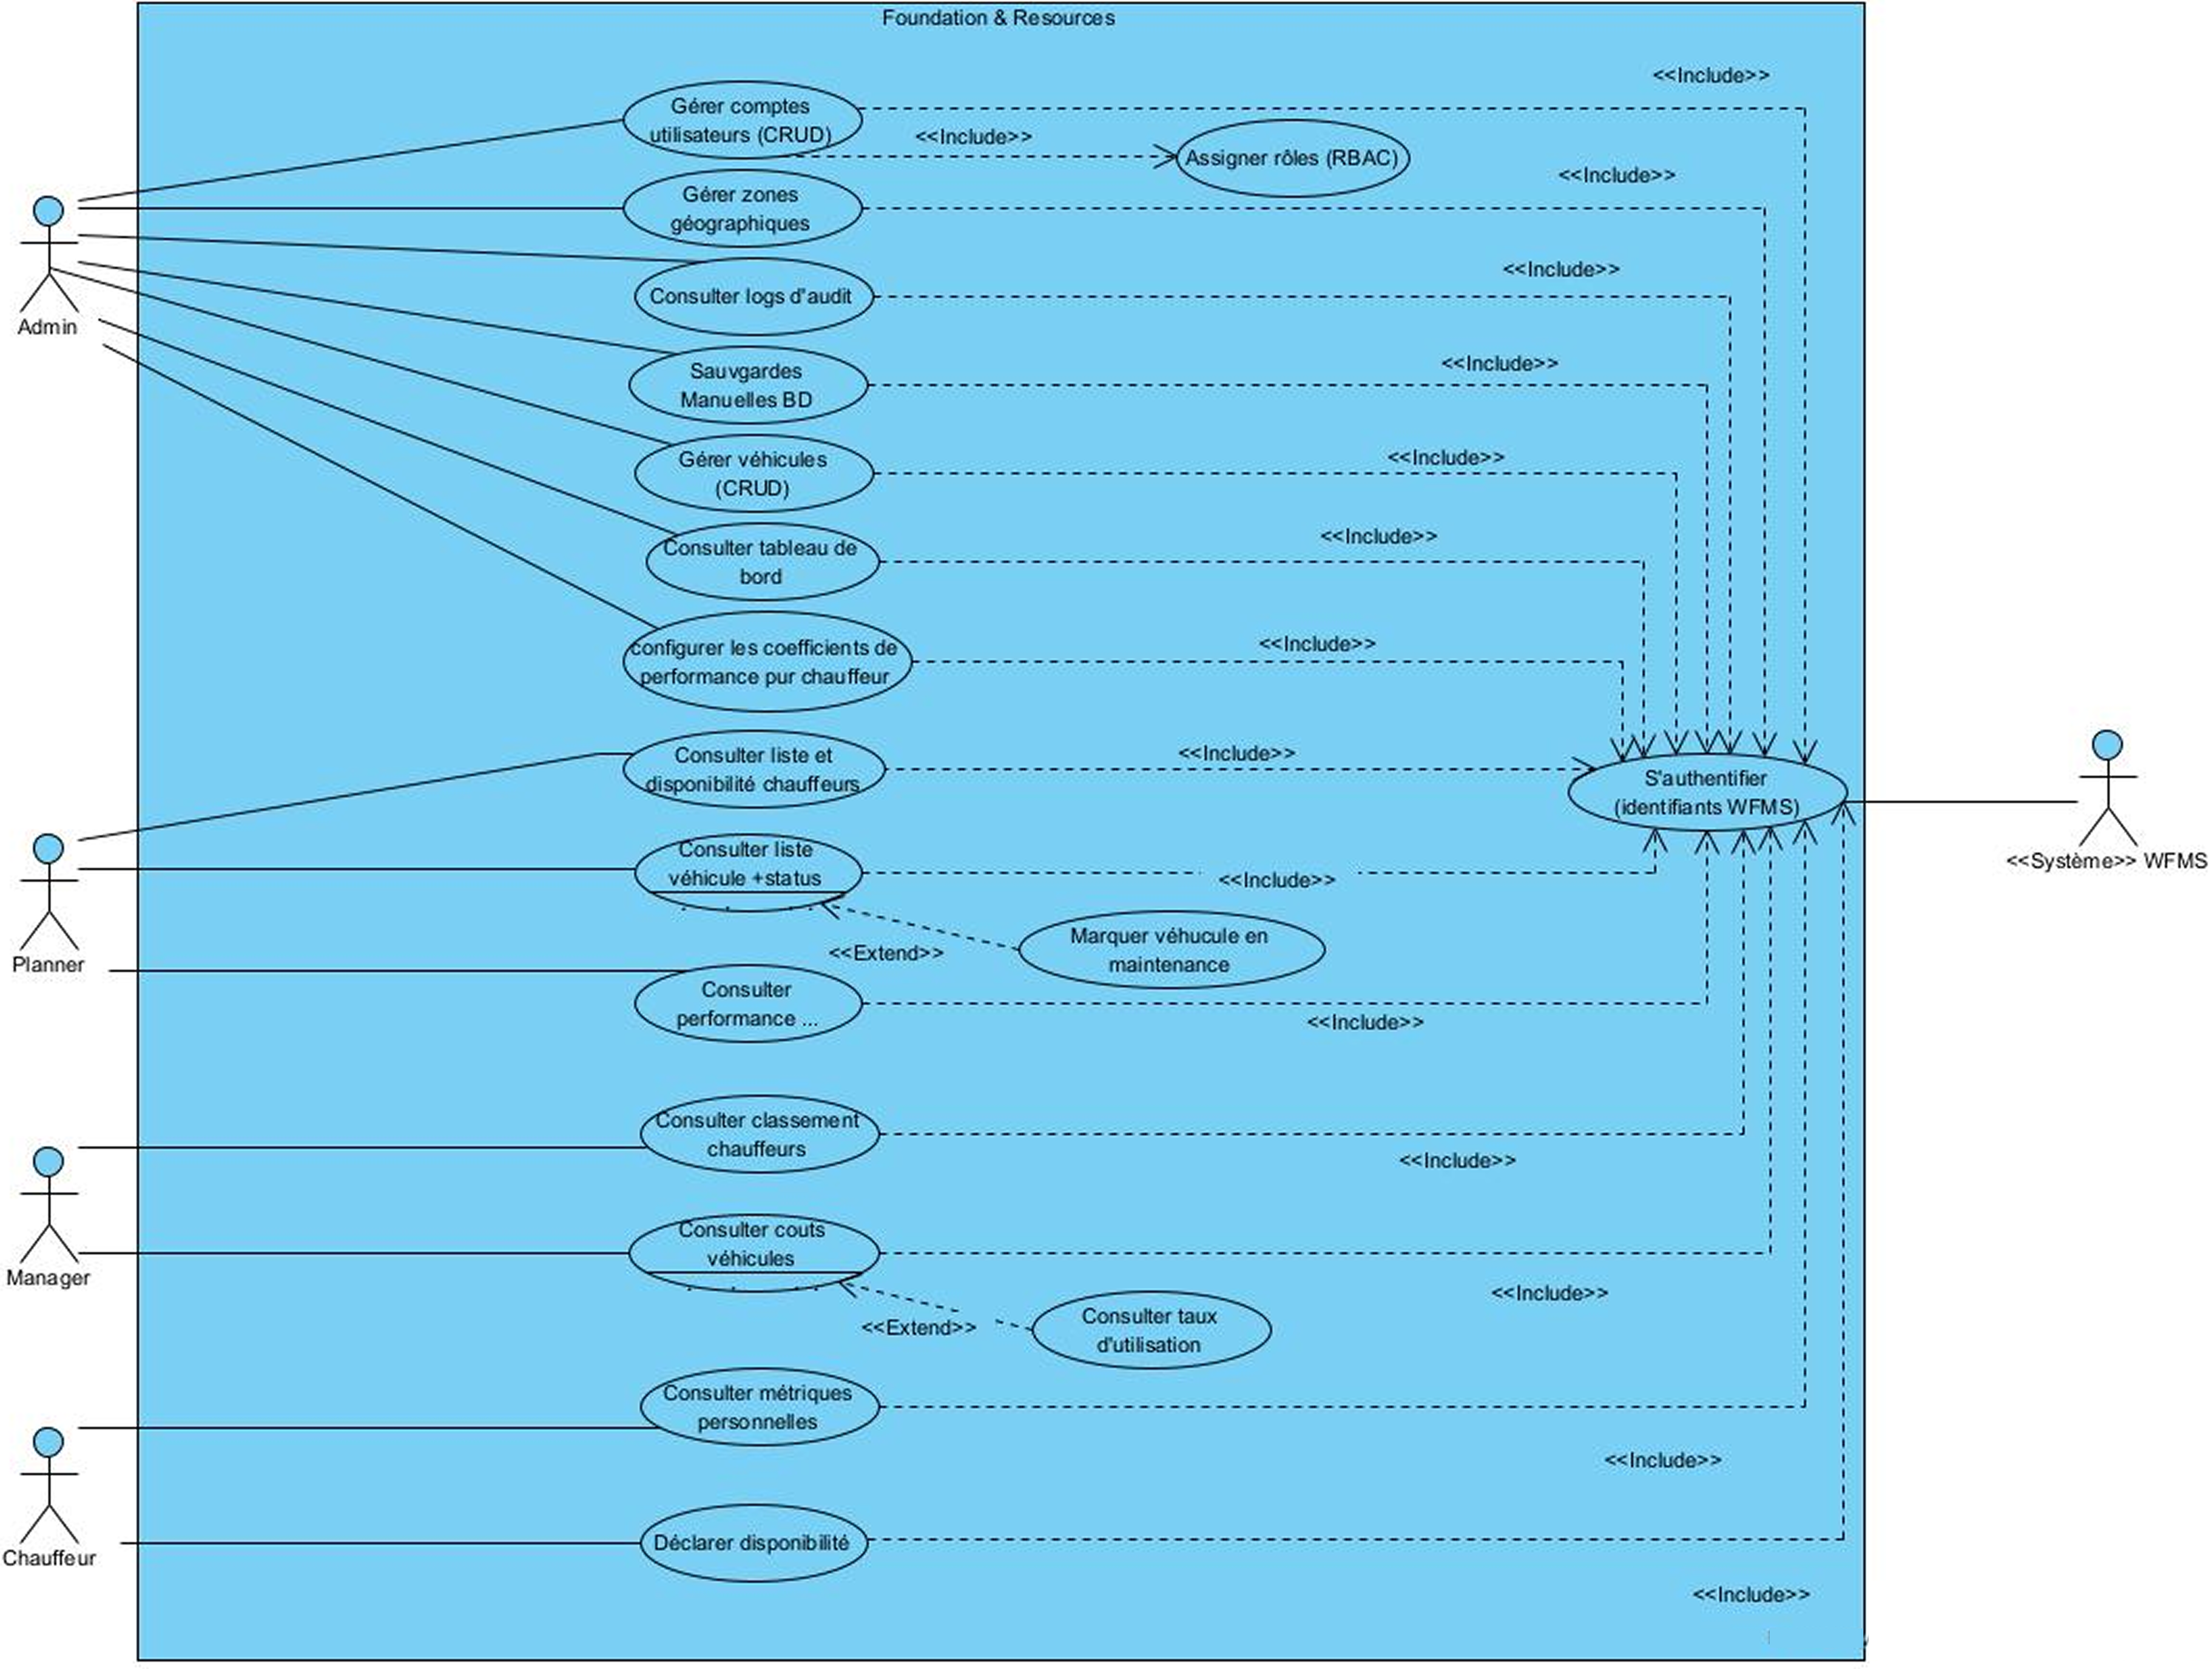
\includegraphics[width=\linewidth, height=0.85\textheight, keepaspectratio]{img/diagrammes/sprint_1_usecase}
\caption{Diagramme de cas d'utilisation du Sprint 1}
\label{fig:cas-utilisation-sp1}
\end{figure}

\subsection{Description textuelle}

\captionsetup[longtable]{justification=centering}
\setlength{\arrayrulewidth}{1pt}
\begin{longtable}{|p{4cm}|p{11cm}|}
\hline
\rowcolor{headerbg}
\textbf{Élément} & \textbf{Description} \\
\hline
\textbf{Titre} & Gérer les chauffeurs \\
\hline
\textbf{Acteurs} & Administrateur, Planificateur \\
\hline
\textbf{Objectif} & Permettre la gestion complète des profils chauffeurs : création, consultation, modification et suppression depuis l'application web. \\
\hline
\textbf{Précondition} & L'utilisateur est authentifié via WFMS et possède le rôle Administrateur ou Planificateur. \\
\hline
\textbf{Postcondition} & L'opération est enregistrée dans le journal d'audit MongoDB. \\
\hline
\textbf{Scénario nominal} &
\begin{enumerate}[start=1, label=\arabic*.]
    \item L'utilisateur accède à la page « Chauffeurs » depuis le menu latéral.
    \item Le système affiche la liste paginée des chauffeurs (nom, prénom, zone, permis, score).
    \item Pour ajouter : l'utilisateur clique sur « Ajouter », remplit le formulaire et valide.
    \item Pour modifier : l'utilisateur clique sur l'icône d'édition, modifie les champs et valide.
    \item Pour supprimer : l'utilisateur clique sur l'icône de suppression et confirme.
    \item Le système enregistre l'opération et met à jour l'affichage.
\end{enumerate} \\
\hline
\textbf{Scénario alternatif} &
\begin{enumerate}[start=1, label=\arabic*.]
    \item Si les données sont invalides (permis expiré, champ vide), un message d'erreur est affiché.
    \item Si l'utilisateur n'a pas le rôle requis, le système retourne une erreur 403.
\end{enumerate} \\
\hline
\caption{Description textuelle --- Gérer les chauffeurs (Sprint 1)}
\end{longtable}
\setlength{\arrayrulewidth}{0.4pt}

\subsection{Diagramme de classes}

\newpage
\thispagestyle{empty}
\begin{landscape}
\begin{figure}[H]
\centering
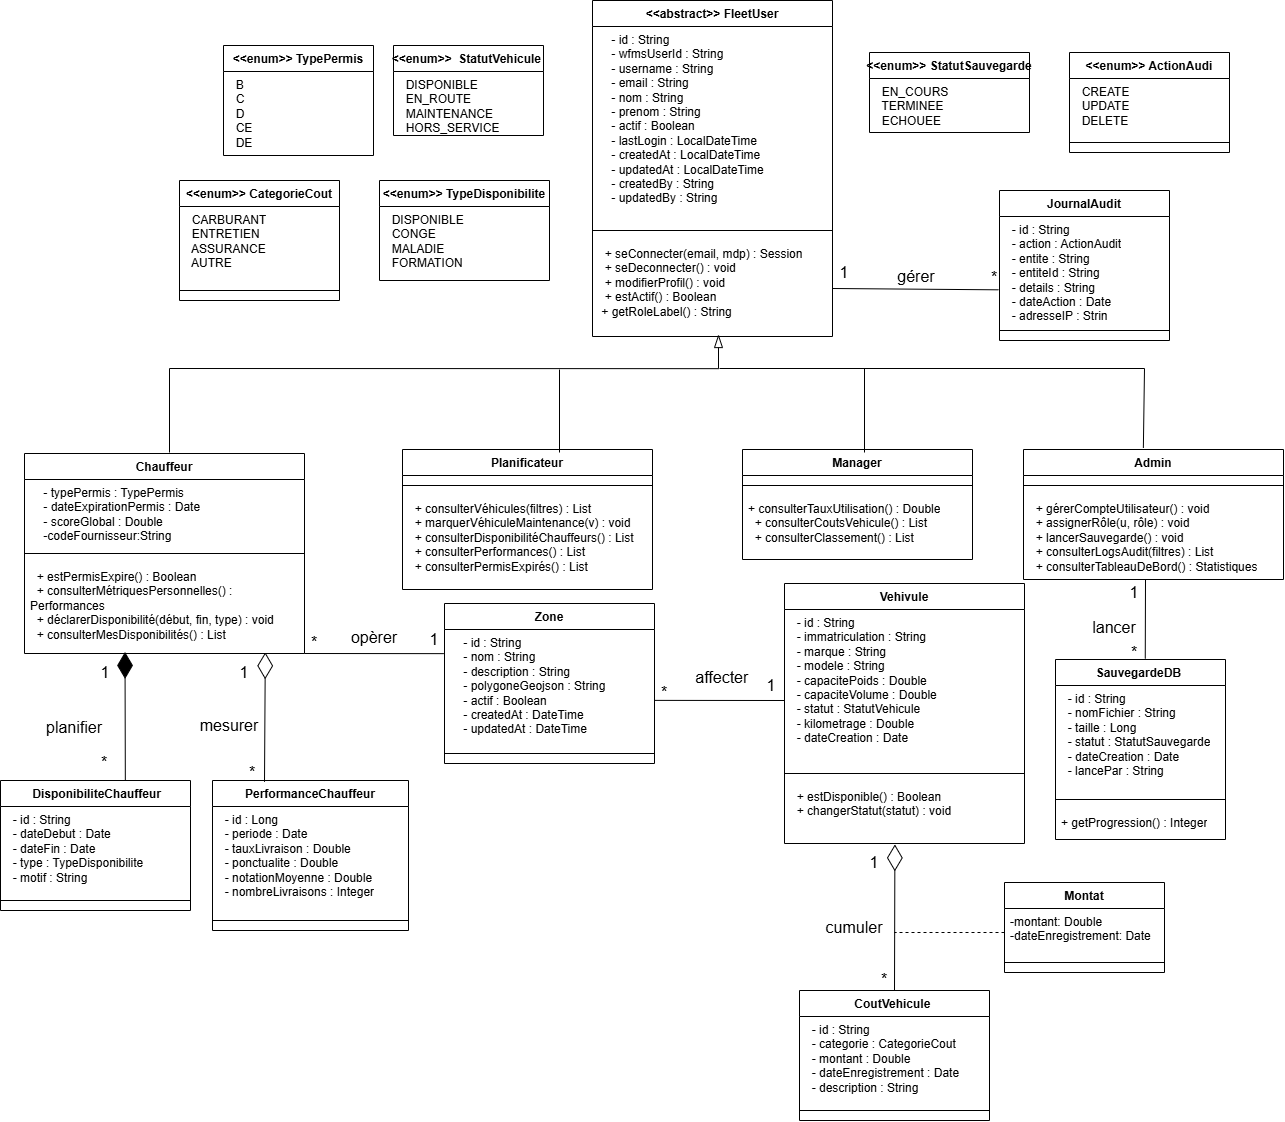
\includegraphics[width=\linewidth, height=0.95\textheight, keepaspectratio]{img/diagrammes/DiagrammeCorrige}
\caption{Diagramme de classes du Sprint 1}
\label{fig:class-diagram-sp1}
\end{figure}
\end{landscape}

% =============================================================
\section{Réalisation}
% =============================================================

\subsection{Sécurité : Authentification et RBAC}
La sécurité applicative repose sur deux composants :
\begin{itemize}
    \item[$\bullet$] \textbf{WfmsAuthFilter :} Filtre qui intercepte les requêtes, déchiffre le token RSA WFMS et injecte l'identité de l'utilisateur.
    \item[$\bullet$] \textbf{RoleInterceptor + @RoleRequired :} Vérifie le rôle requis via l'héritage polymorphique des entités FleetUser.
\end{itemize}

\subsection{Tableau de bord et authentification}

L'authentification passe par WFMS. Chaque acteur est redirigé vers son tableau de bord avec KPIs en temps réel.

\begin{figure}[H]
\centering
\IfFileExists{img/capture/web/sp1_dashboard_composite.png}{%
  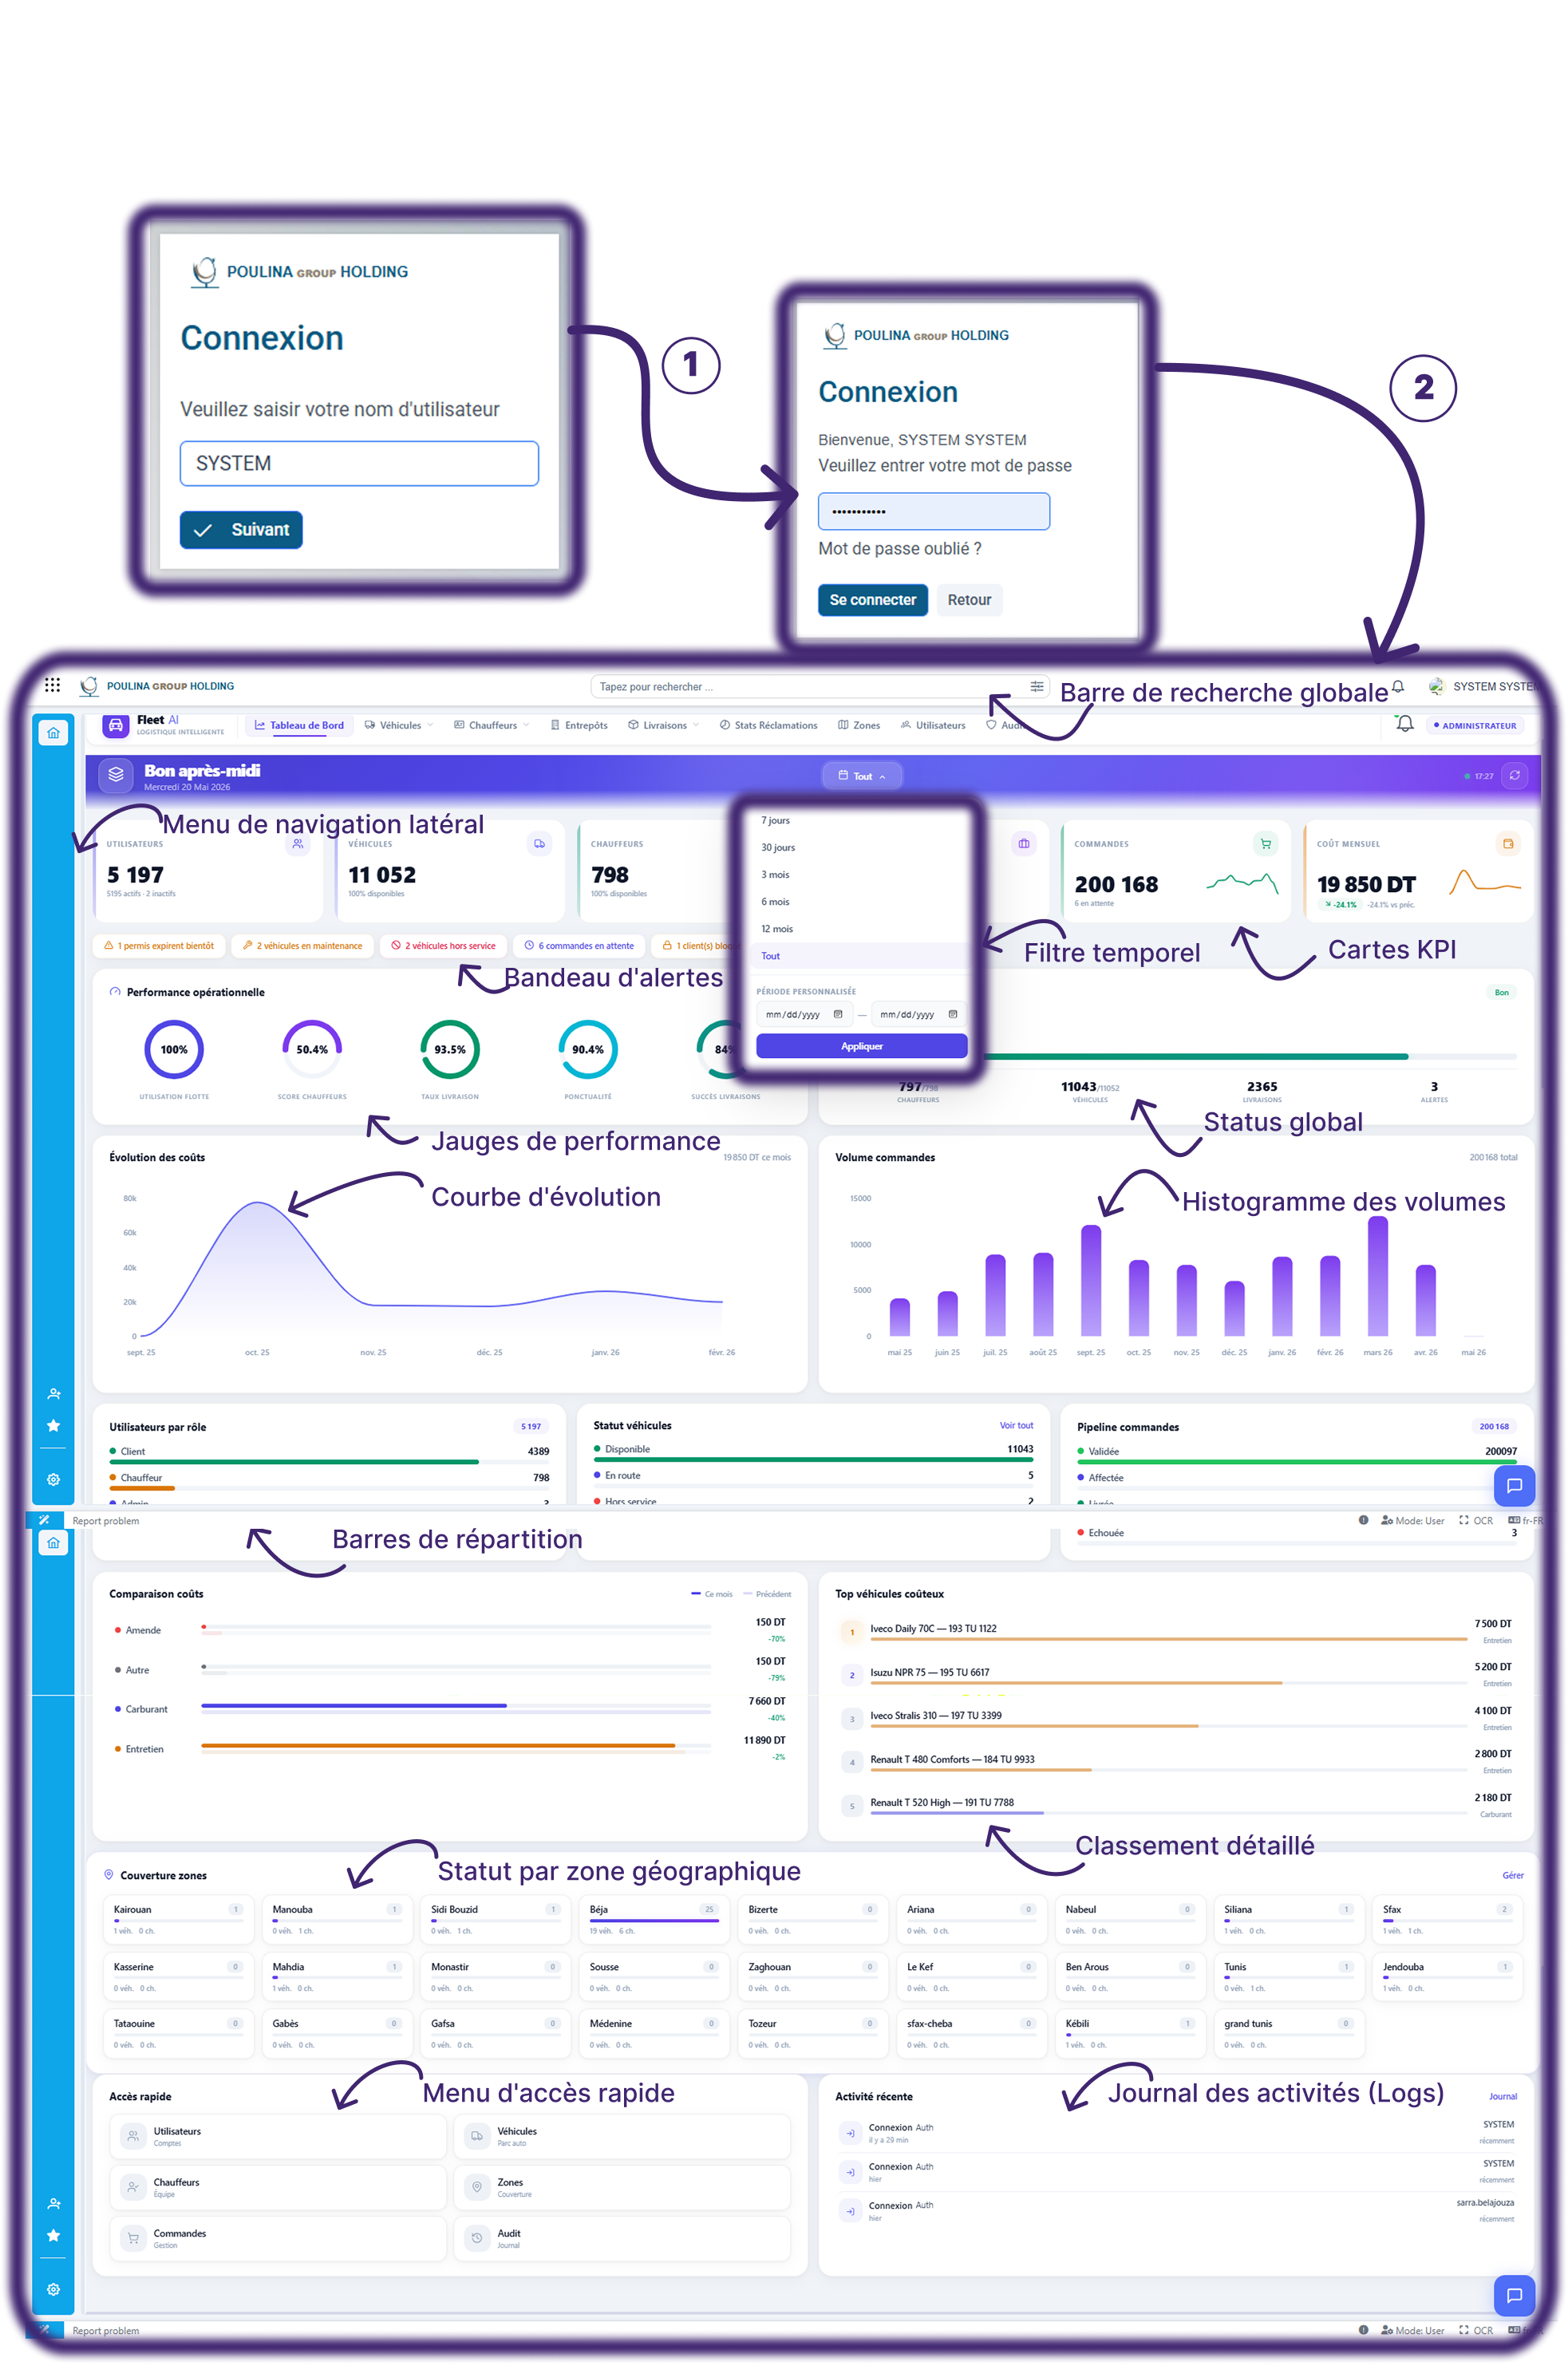
\includegraphics[width=\linewidth, keepaspectratio]{img/capture/web/sp1_dashboard_composite}%
}{%
  \fbox{\parbox{0.9\linewidth}{\centering\vspace{4cm}\textit{[img/sp1\_dashboard\_composite]}\vspace{4cm}}}%
}
\caption{Tableau de bord Fleet~AI : KPIs administrateur et connexion WFMS}
\label{fig:sp1-dashboard}
\end{figure}

\subsection{Gestion des utilisateurs}

L'Administrateur crée, modifie et désactive des comptes utilisateurs, en assignant l'un des six rôles disponibles : AD, MG, PL, CH, REC, CL. Un compte désactivé perd immédiatement tout accès.

\begin{figure}[H]
\centering
\IfFileExists{img/capture/web/sp1_users_composite.png}{%
  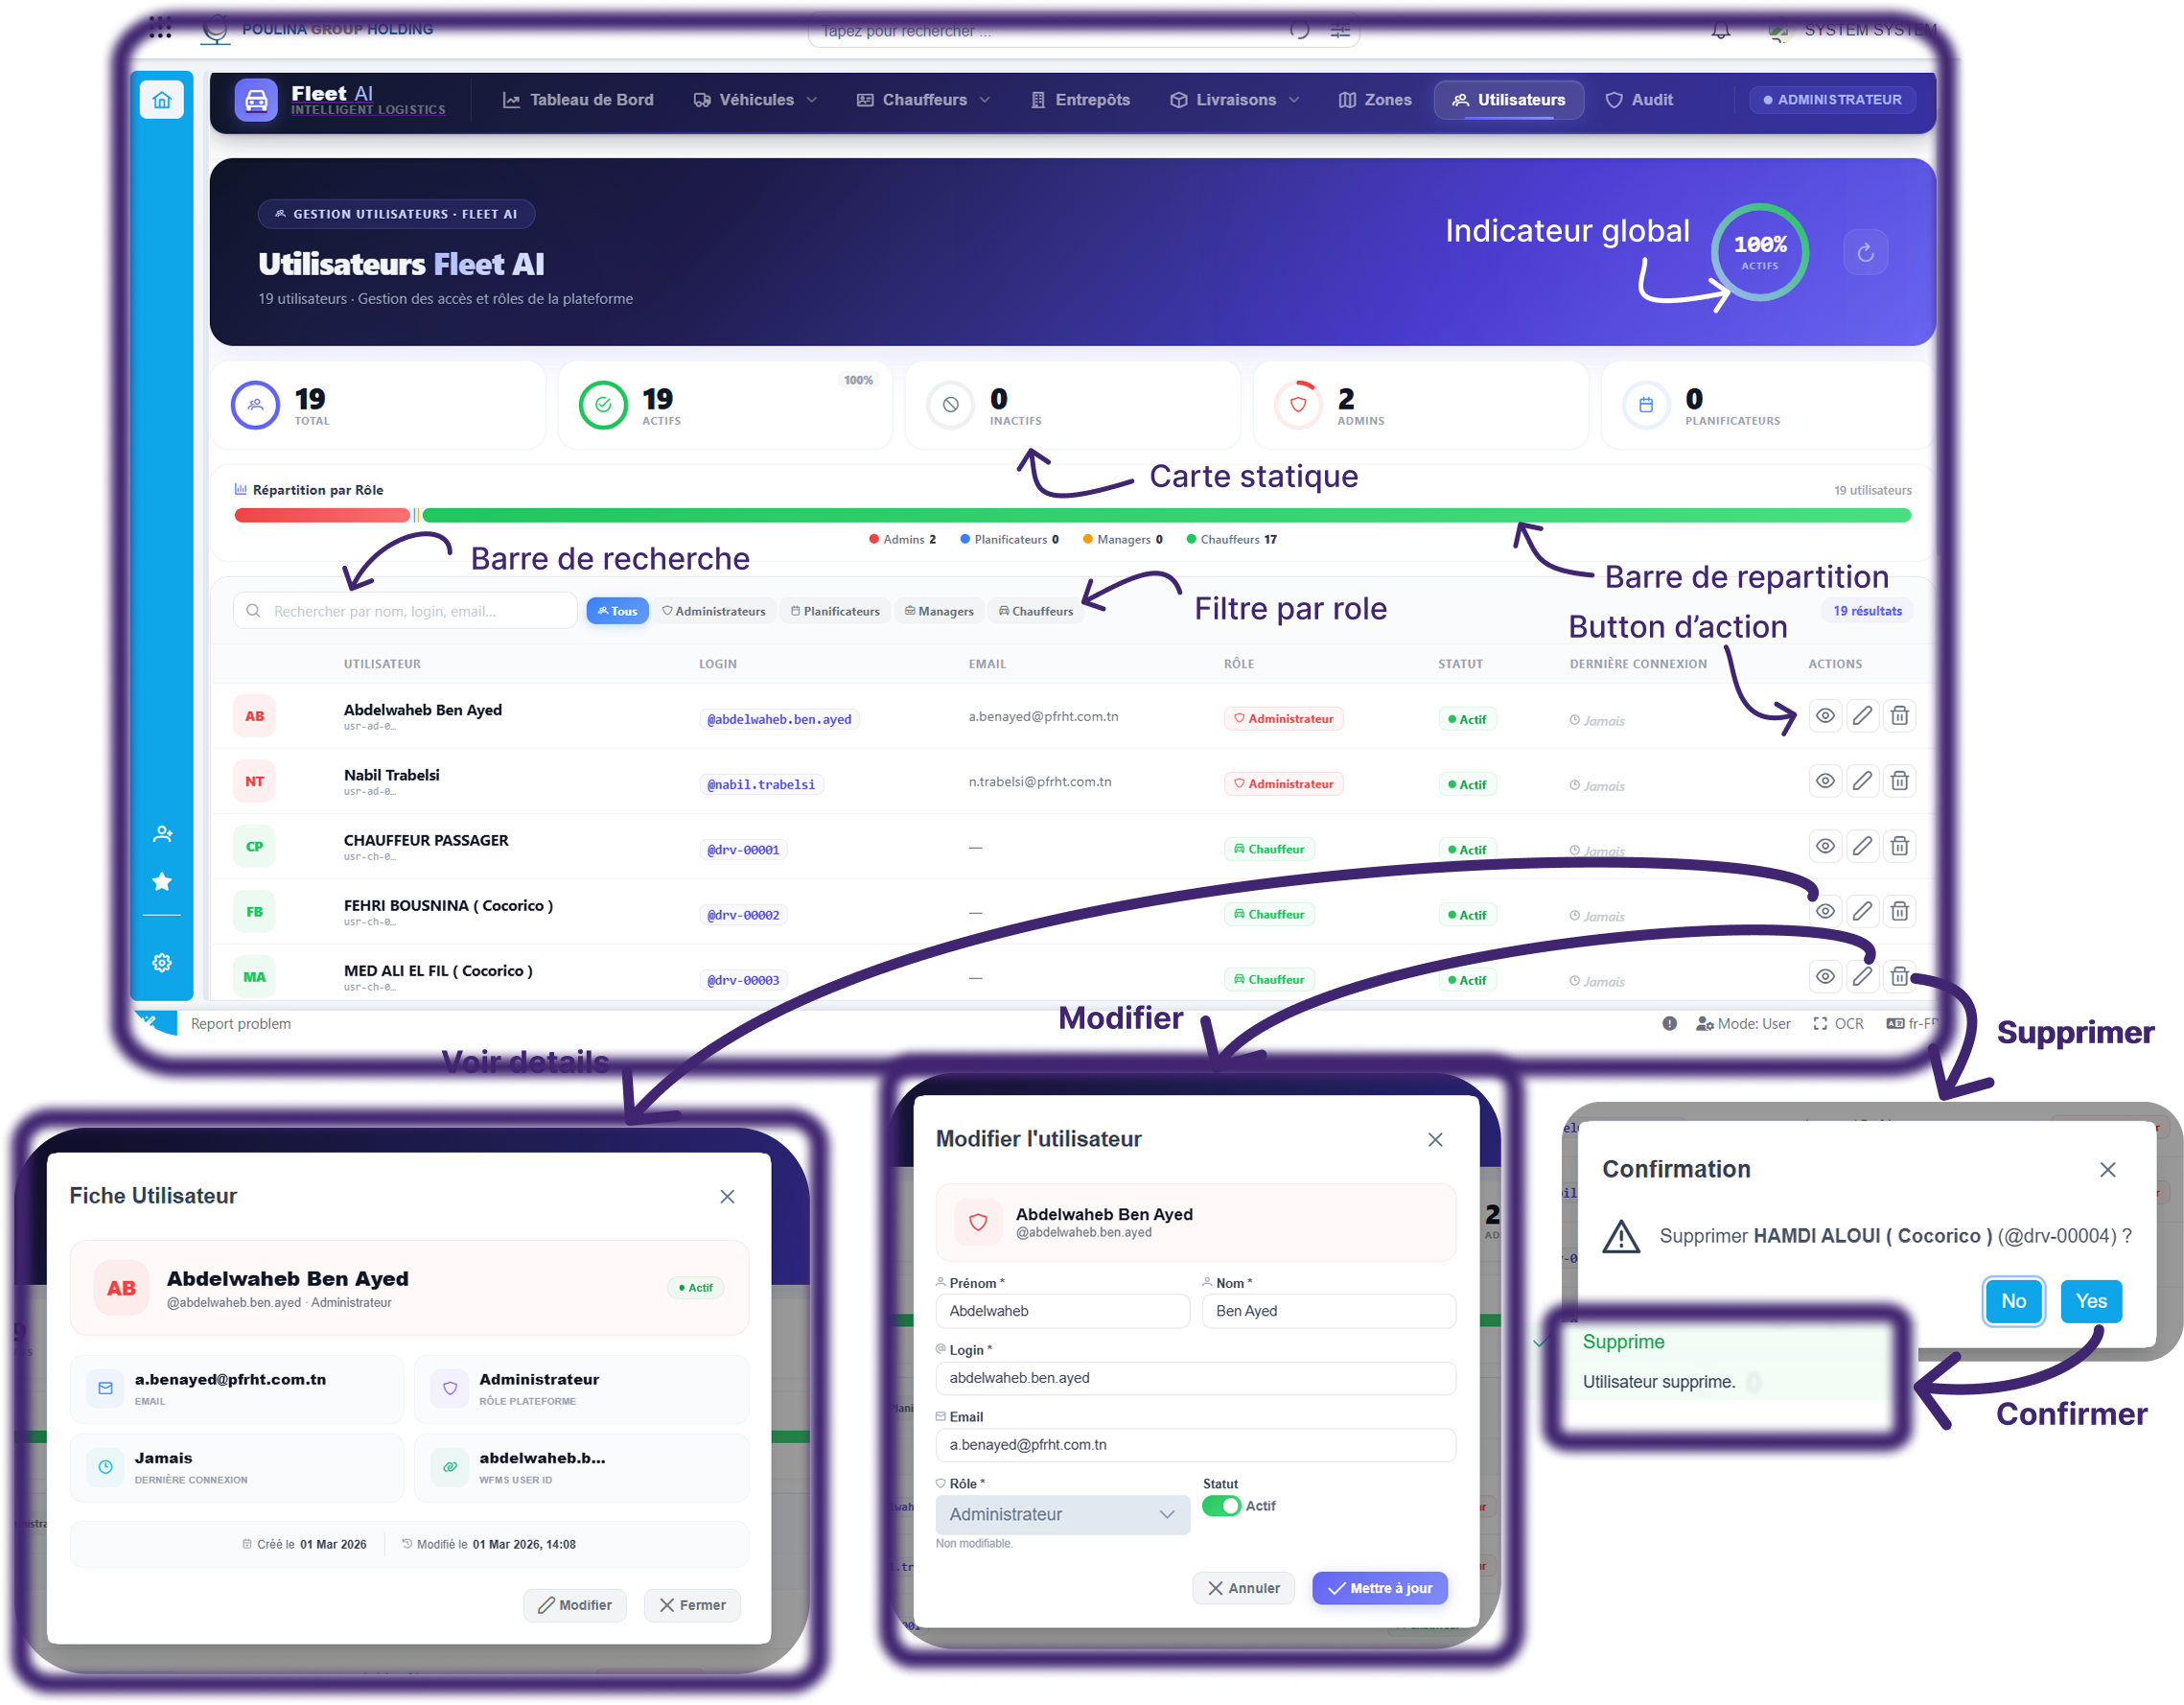
\includegraphics[width=\linewidth, keepaspectratio]{img/capture/web/sp1_users_composite}%
}{%
  \fbox{\parbox{0.9\linewidth}{\centering\vspace{4cm}\textit{[img/sp1\_users\_composite]}\vspace{4cm}}}%
}
\caption{Gestion des utilisateurs : liste par rôle et formulaire de création}
\label{fig:sp1-users}
\end{figure}

\subsection{Gestion des véhicules}

Chaque véhicule est défini par son immatriculation, ses capacités (poids, volume), son statut et sa zone d'affectation. Le suivi des coûts et de l'historique kilométrique est intégré.

\begin{figure}[H]
\centering
\IfFileExists{img/capture/web/sp1_vehicles_composite.png}{%
  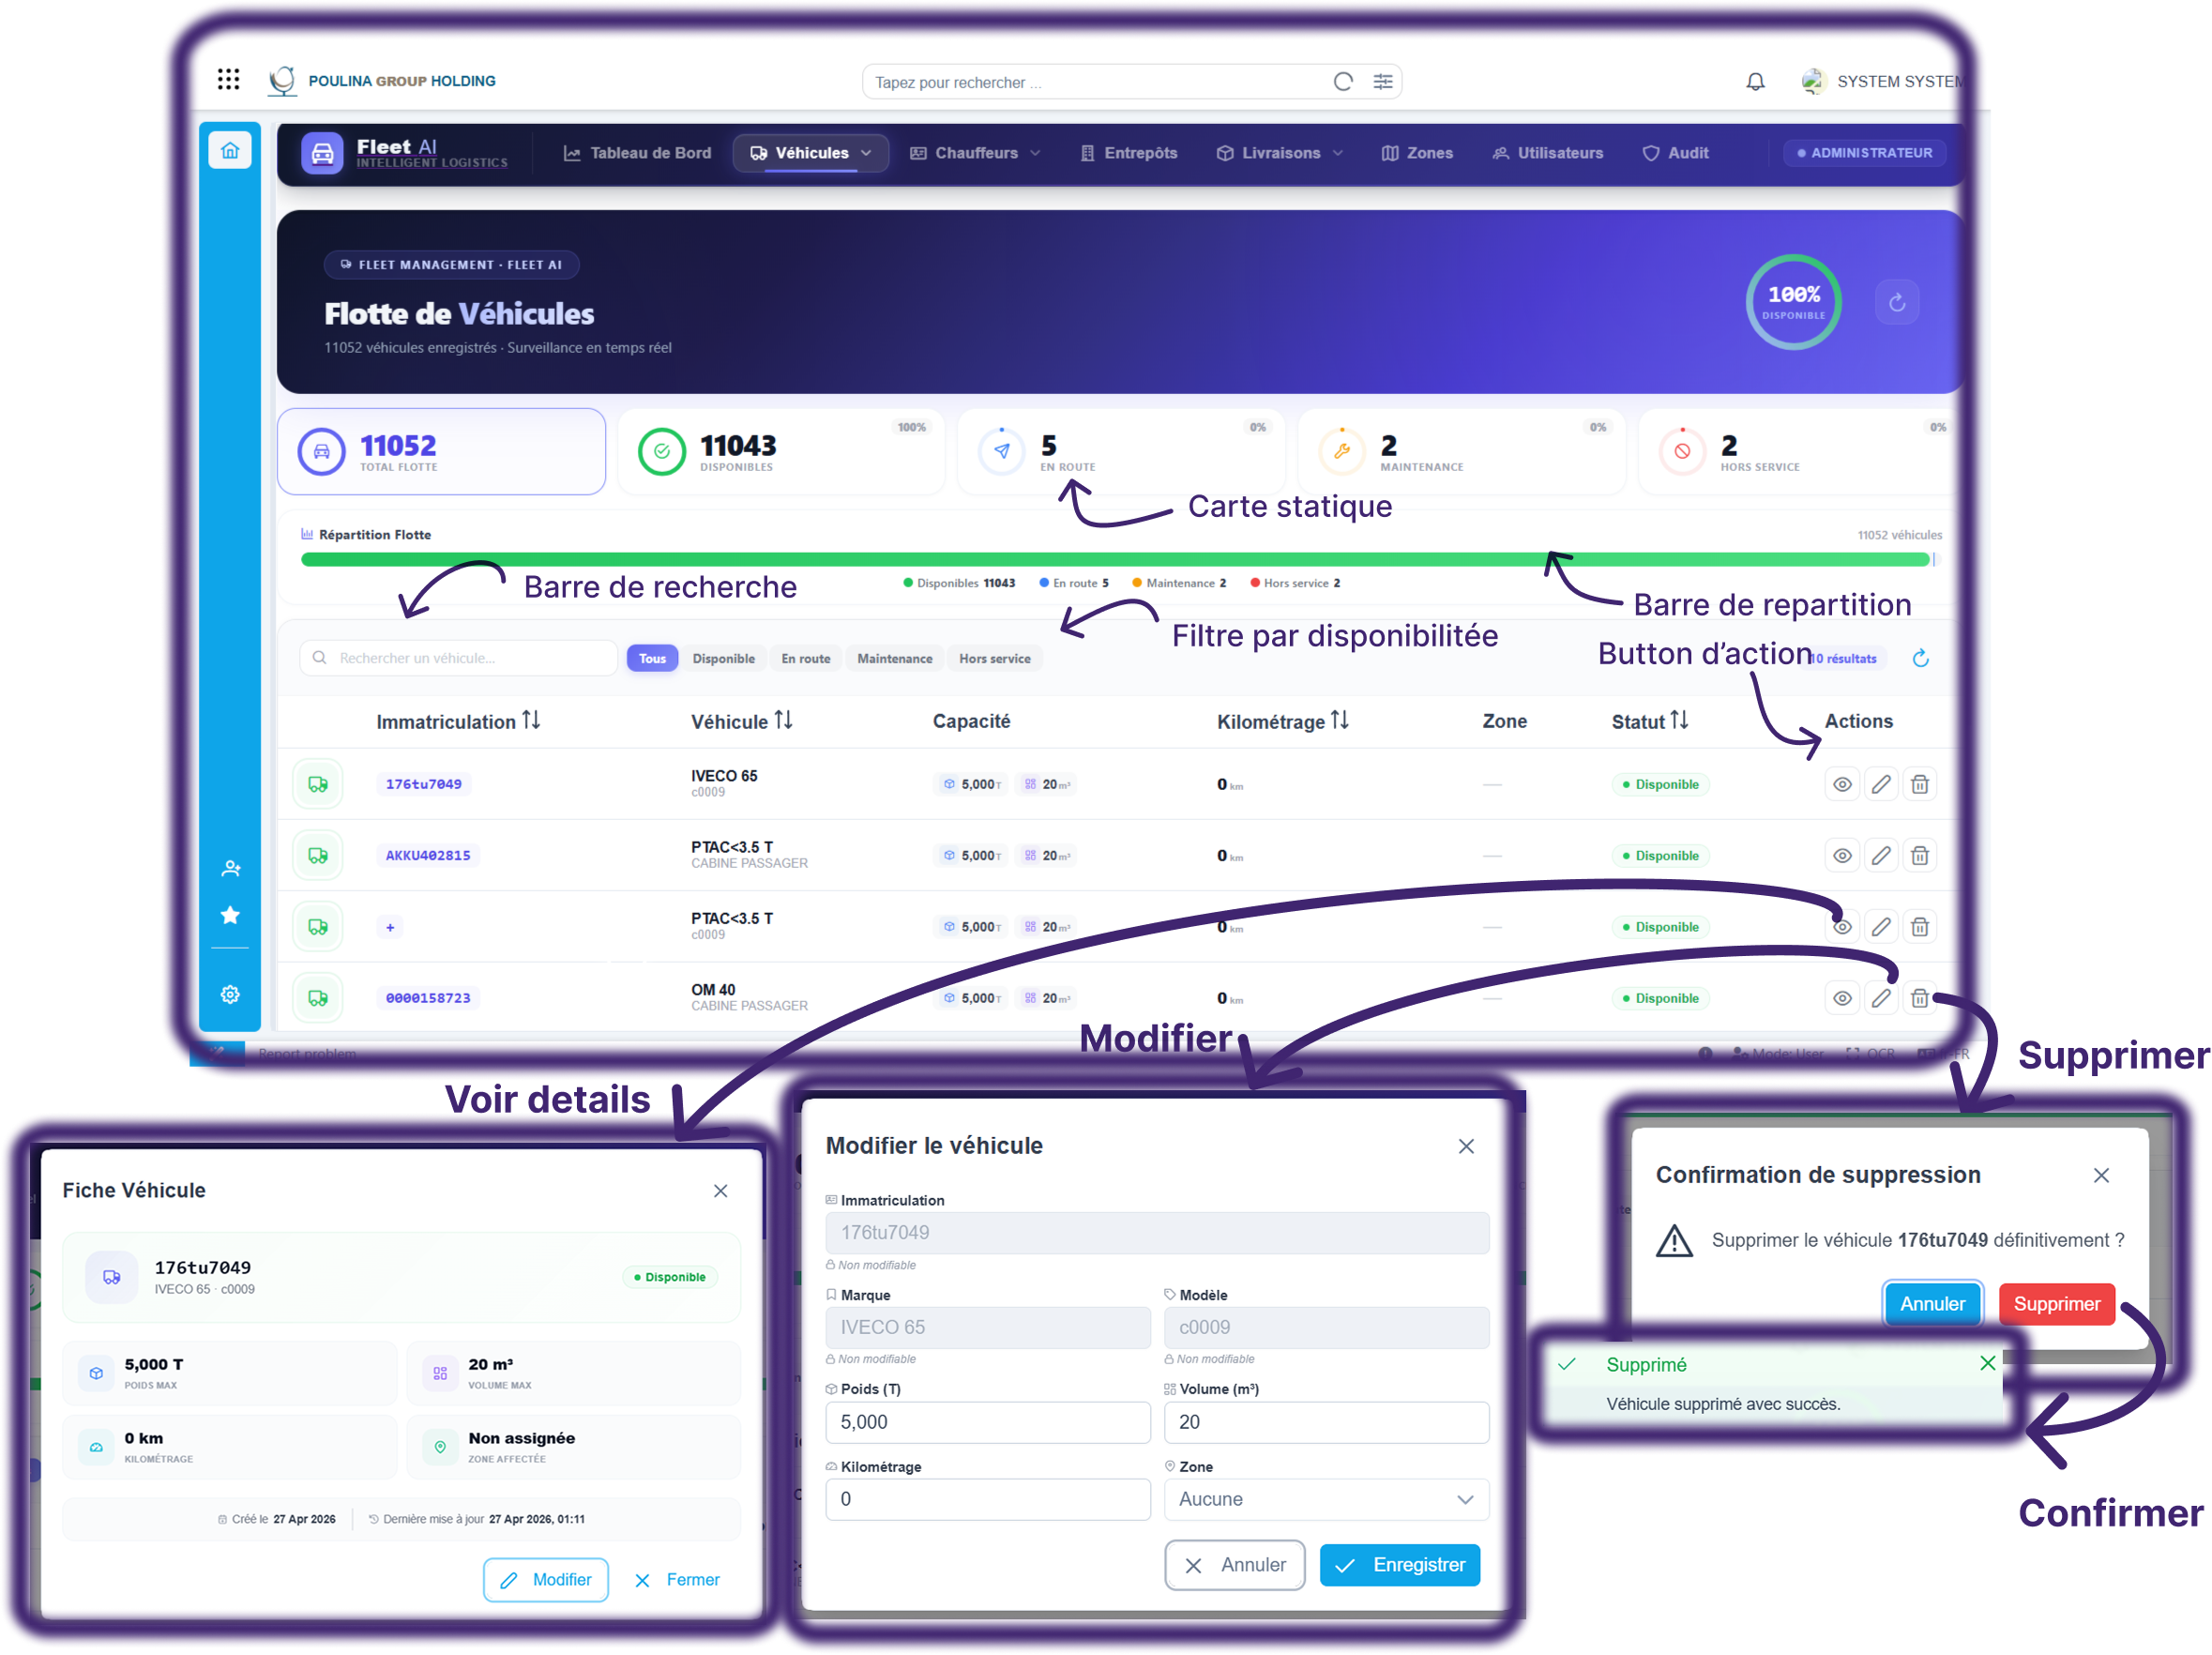
\includegraphics[width=\linewidth, keepaspectratio]{img/capture/web/sp1_vehicles_composite}%
}{%
  \fbox{\parbox{0.9\linewidth}{\centering\vspace{4cm}\textit{[img/sp1\_vehicles\_composite]}\vspace{4cm}}}%
}
\caption{Gestion des véhicules : statuts, capacités et formulaire d'ajout}
\label{fig:sp1-vehicles}
\end{figure}

\subsection{Gestion des chauffeurs}

Le cycle de vie complet est couvert : création avec type de permis (B, C, CE, D, DE), zone d'affectation et contrat (Officiel / Prestataire). Le score global est calculé automatiquement à partir de trois coefficients configurables.

\begin{figure}[H]
\centering
\IfFileExists{img/capture/web/sp1_drivers_composite.png}{%
  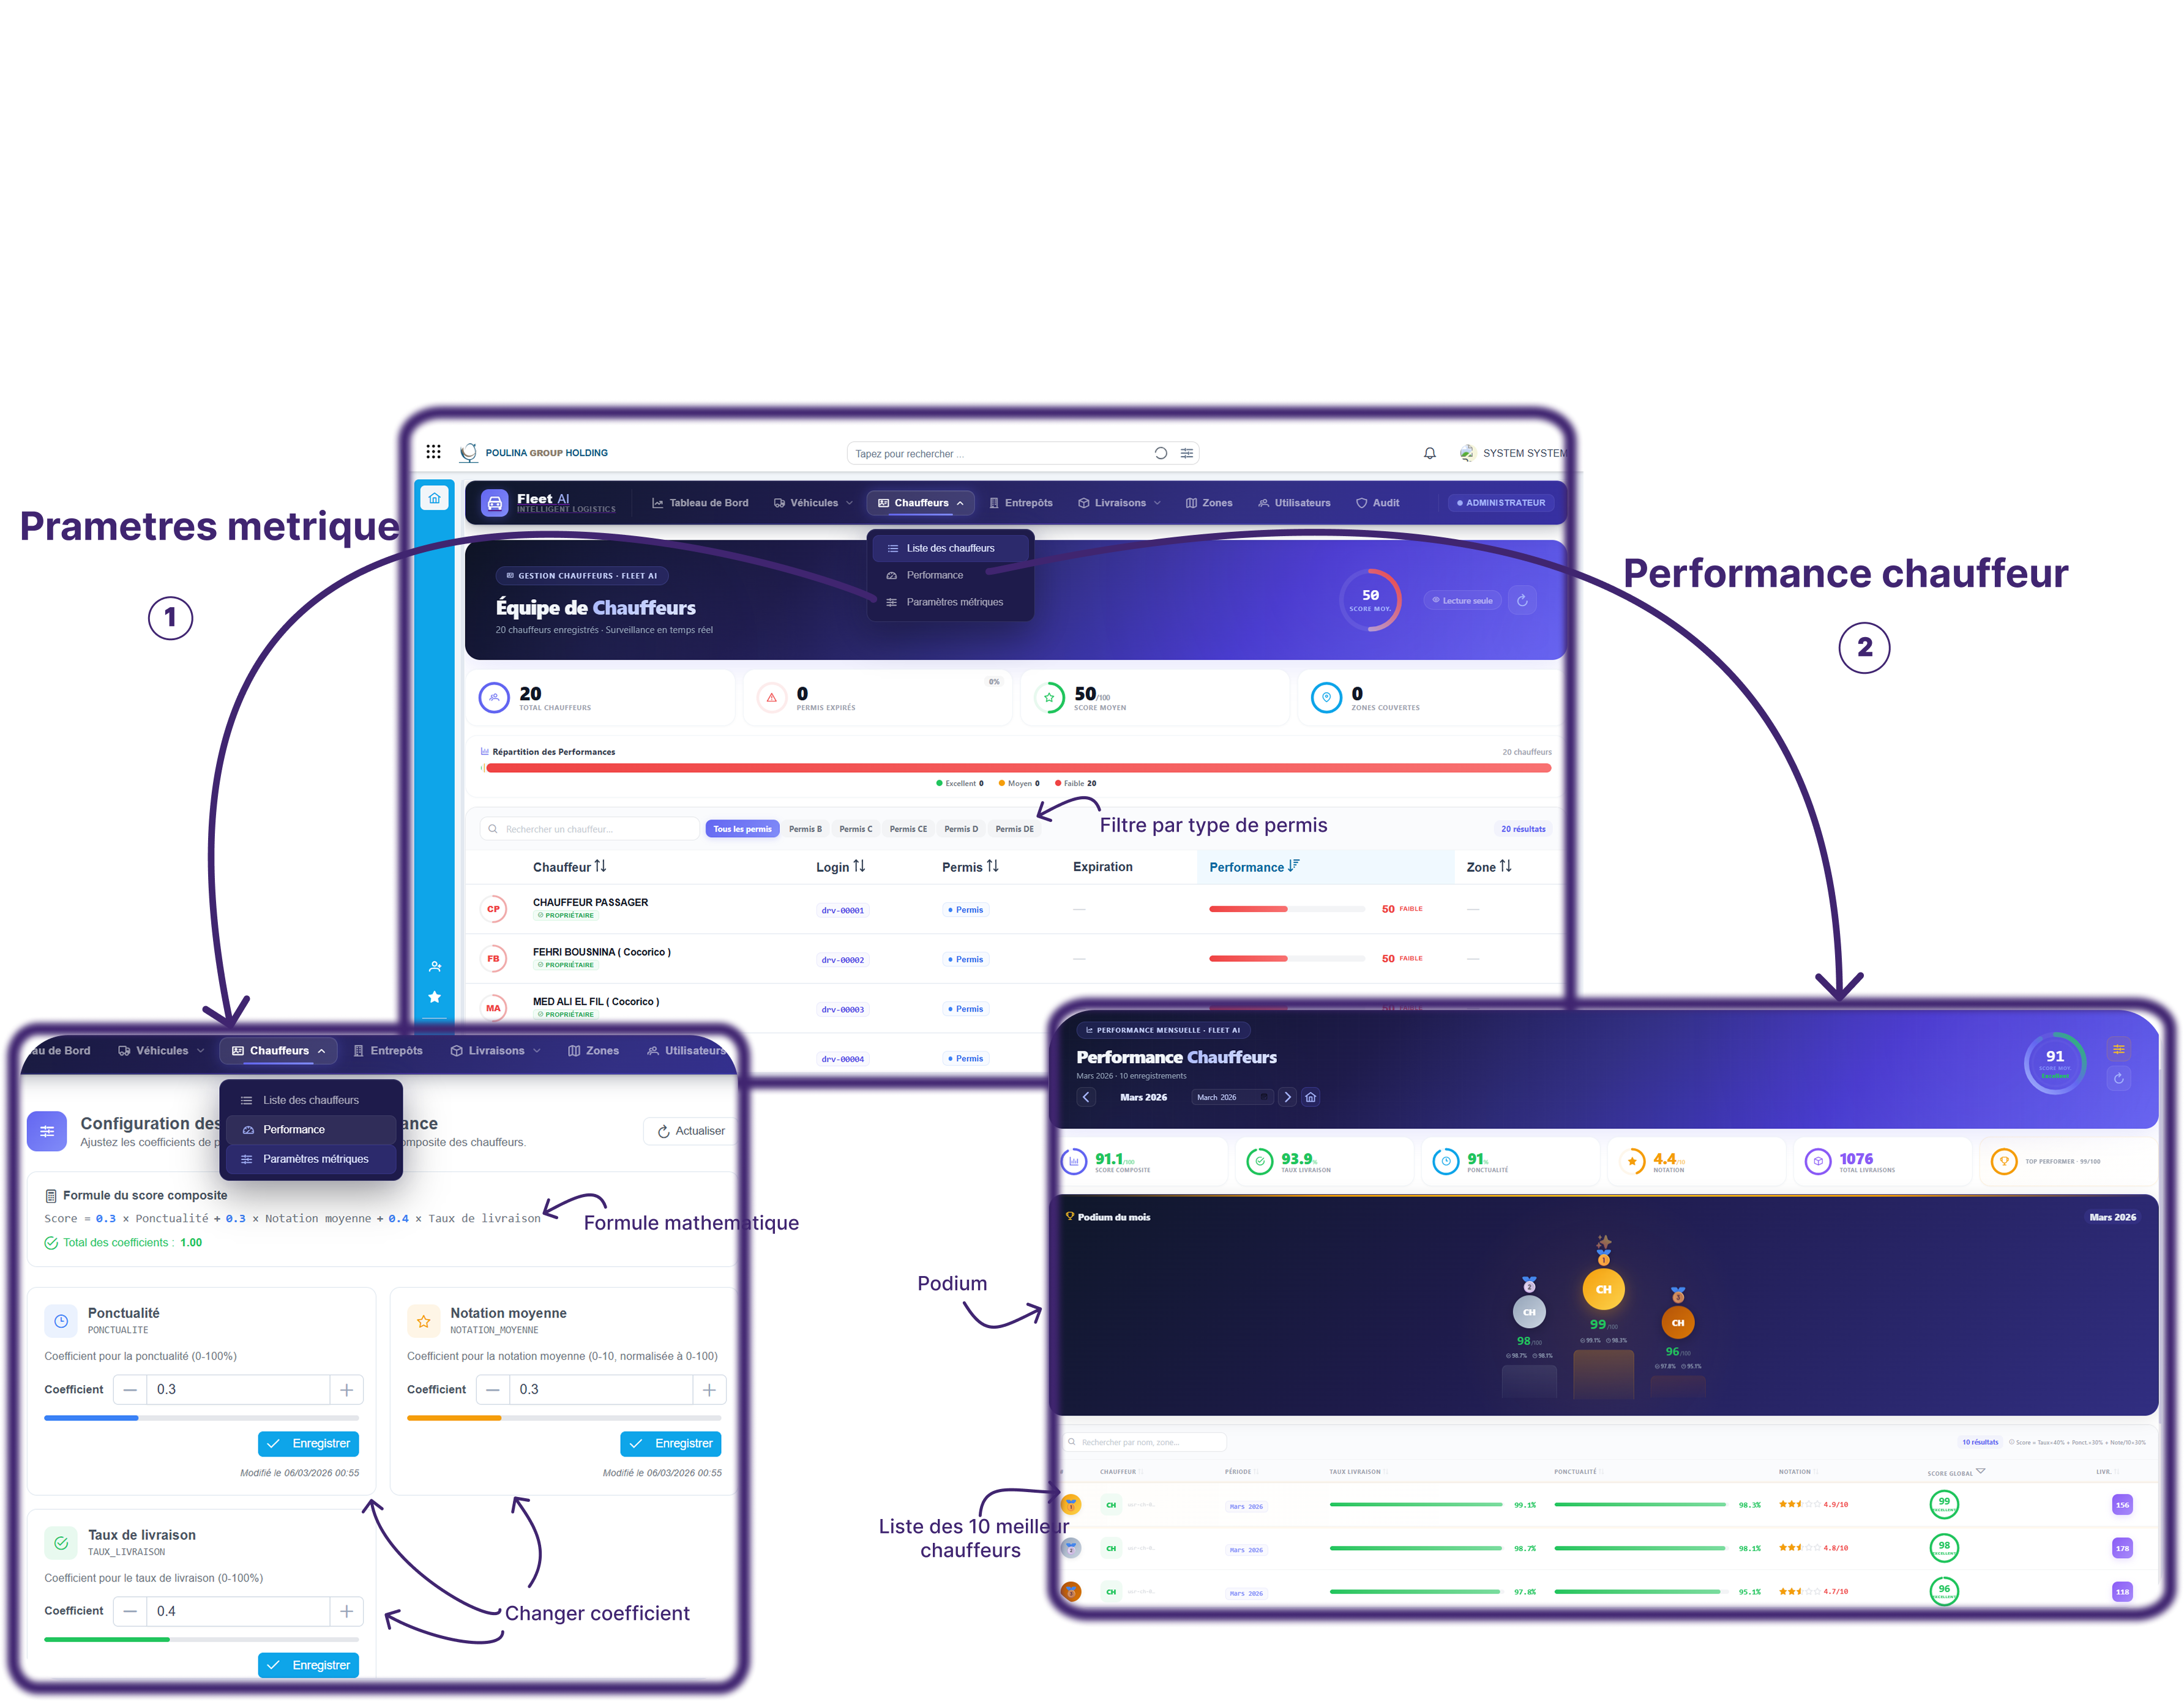
\includegraphics[width=\linewidth, keepaspectratio]{img/capture/web/sp1_drivers_composite}%
}{%
  \fbox{\parbox{0.9\linewidth}{\centering\vspace{4cm}\textit{[img/sp1\_drivers\_composite]}\vspace{4cm}}}%
}
\caption{Gestion des chauffeurs : score, performance et type de permis}
\label{fig:sp1-drivers}
\end{figure}

\subsection{Gestion des zones géographiques}

La gestion des zones permet de définir les périmètres de livraison. Deux types de zones sont supportés : \texttt{STATE\_BASED} (24 gouvernorats tunisiens) et \texttt{MANUAL\_POLYGON} (zones dessinées librement sur carte Leaflet). La détection automatique de zone s'effectue lors de l'ajout d'une adresse client.

\begin{figure}[H]
\centering
\IfFileExists{img/capture/web/sp1_zones_composite.png}{%
  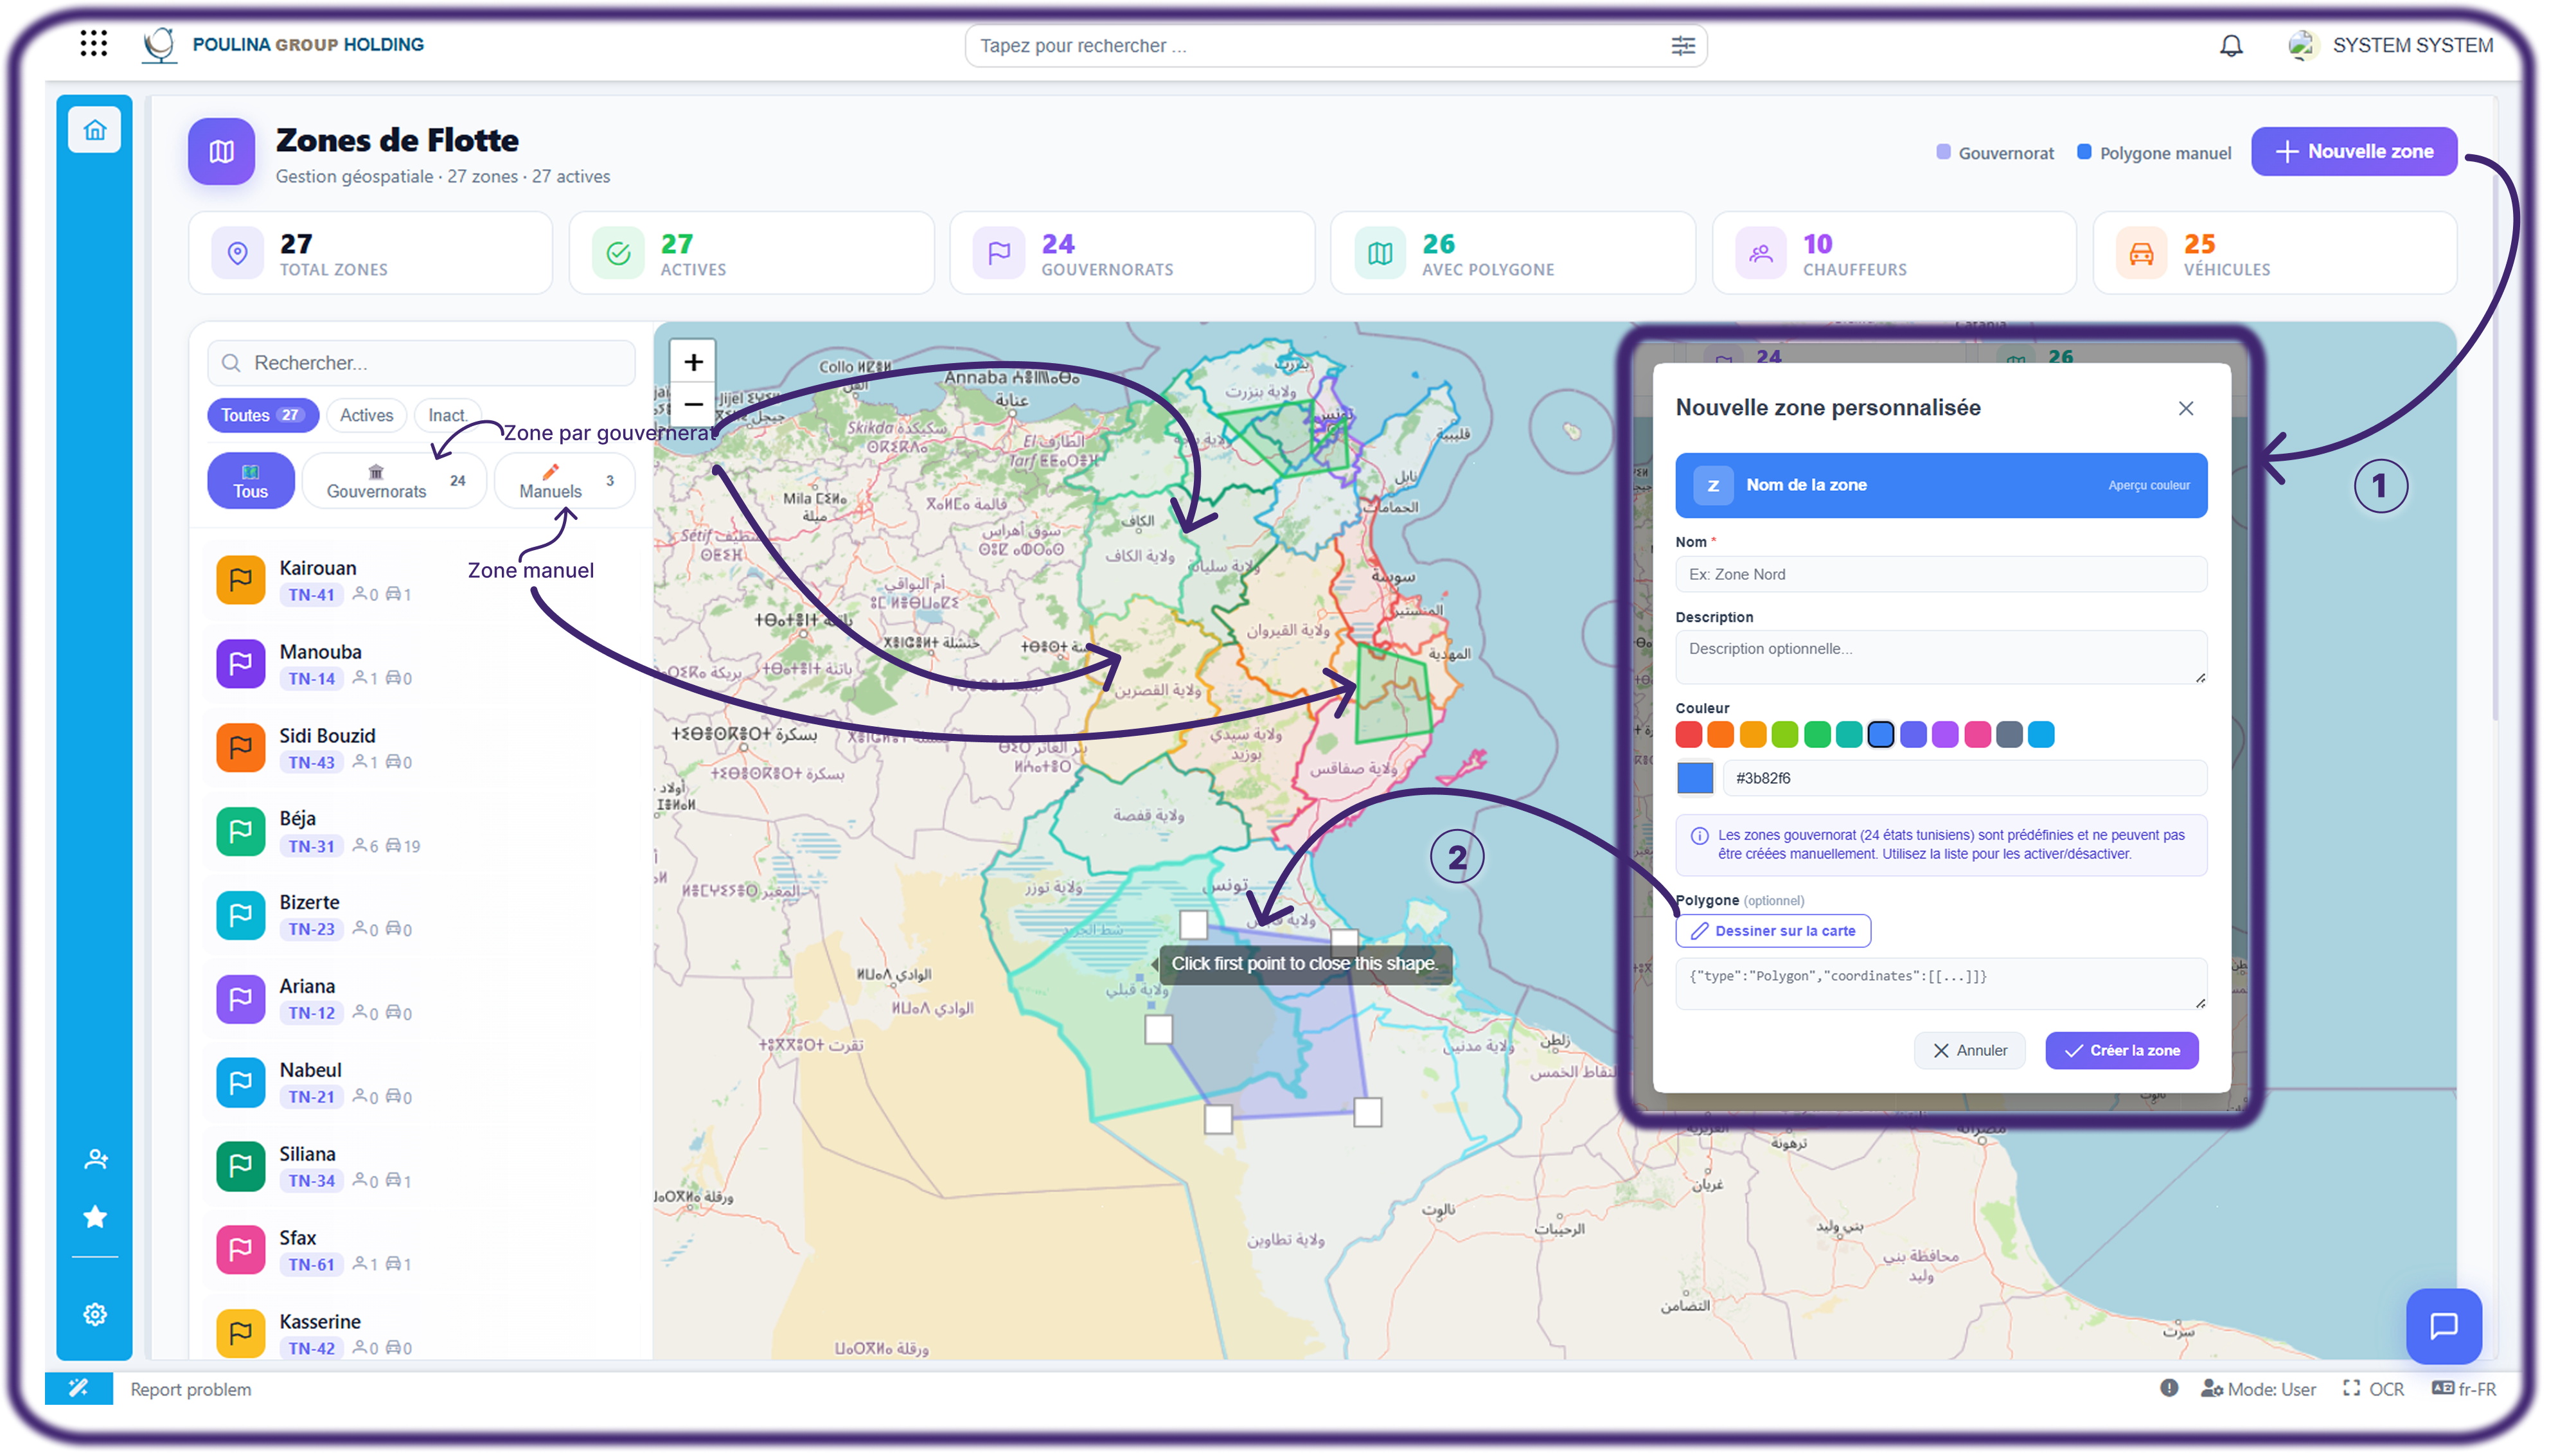
\includegraphics[width=\linewidth, keepaspectratio]{img/capture/web/sp1_zones_composite}%
}{%
  \fbox{\parbox{0.9\linewidth}{\centering\vspace{4cm}\textit{[img/sp1\_zones\_composite]}\vspace{4cm}}}%
}
\caption{Gestion des zones : périmètres et éditeur de polygone Leaflet}
\label{fig:sp1-zones}
\end{figure}

\subsection{Journal d'audit et sauvegardes}

Toutes les actions critiques sont enregistrées automatiquement dans le journal d'audit avec double stockage PostgreSQL et MongoDB. L'Administrateur filtre le journal par date, utilisateur et action. La fonctionnalité de sauvegarde déclenche une copie complète de la base.

\begin{figure}[H]
\centering
\IfFileExists{img/capture/web/sp1_audit_composite.png}{%
  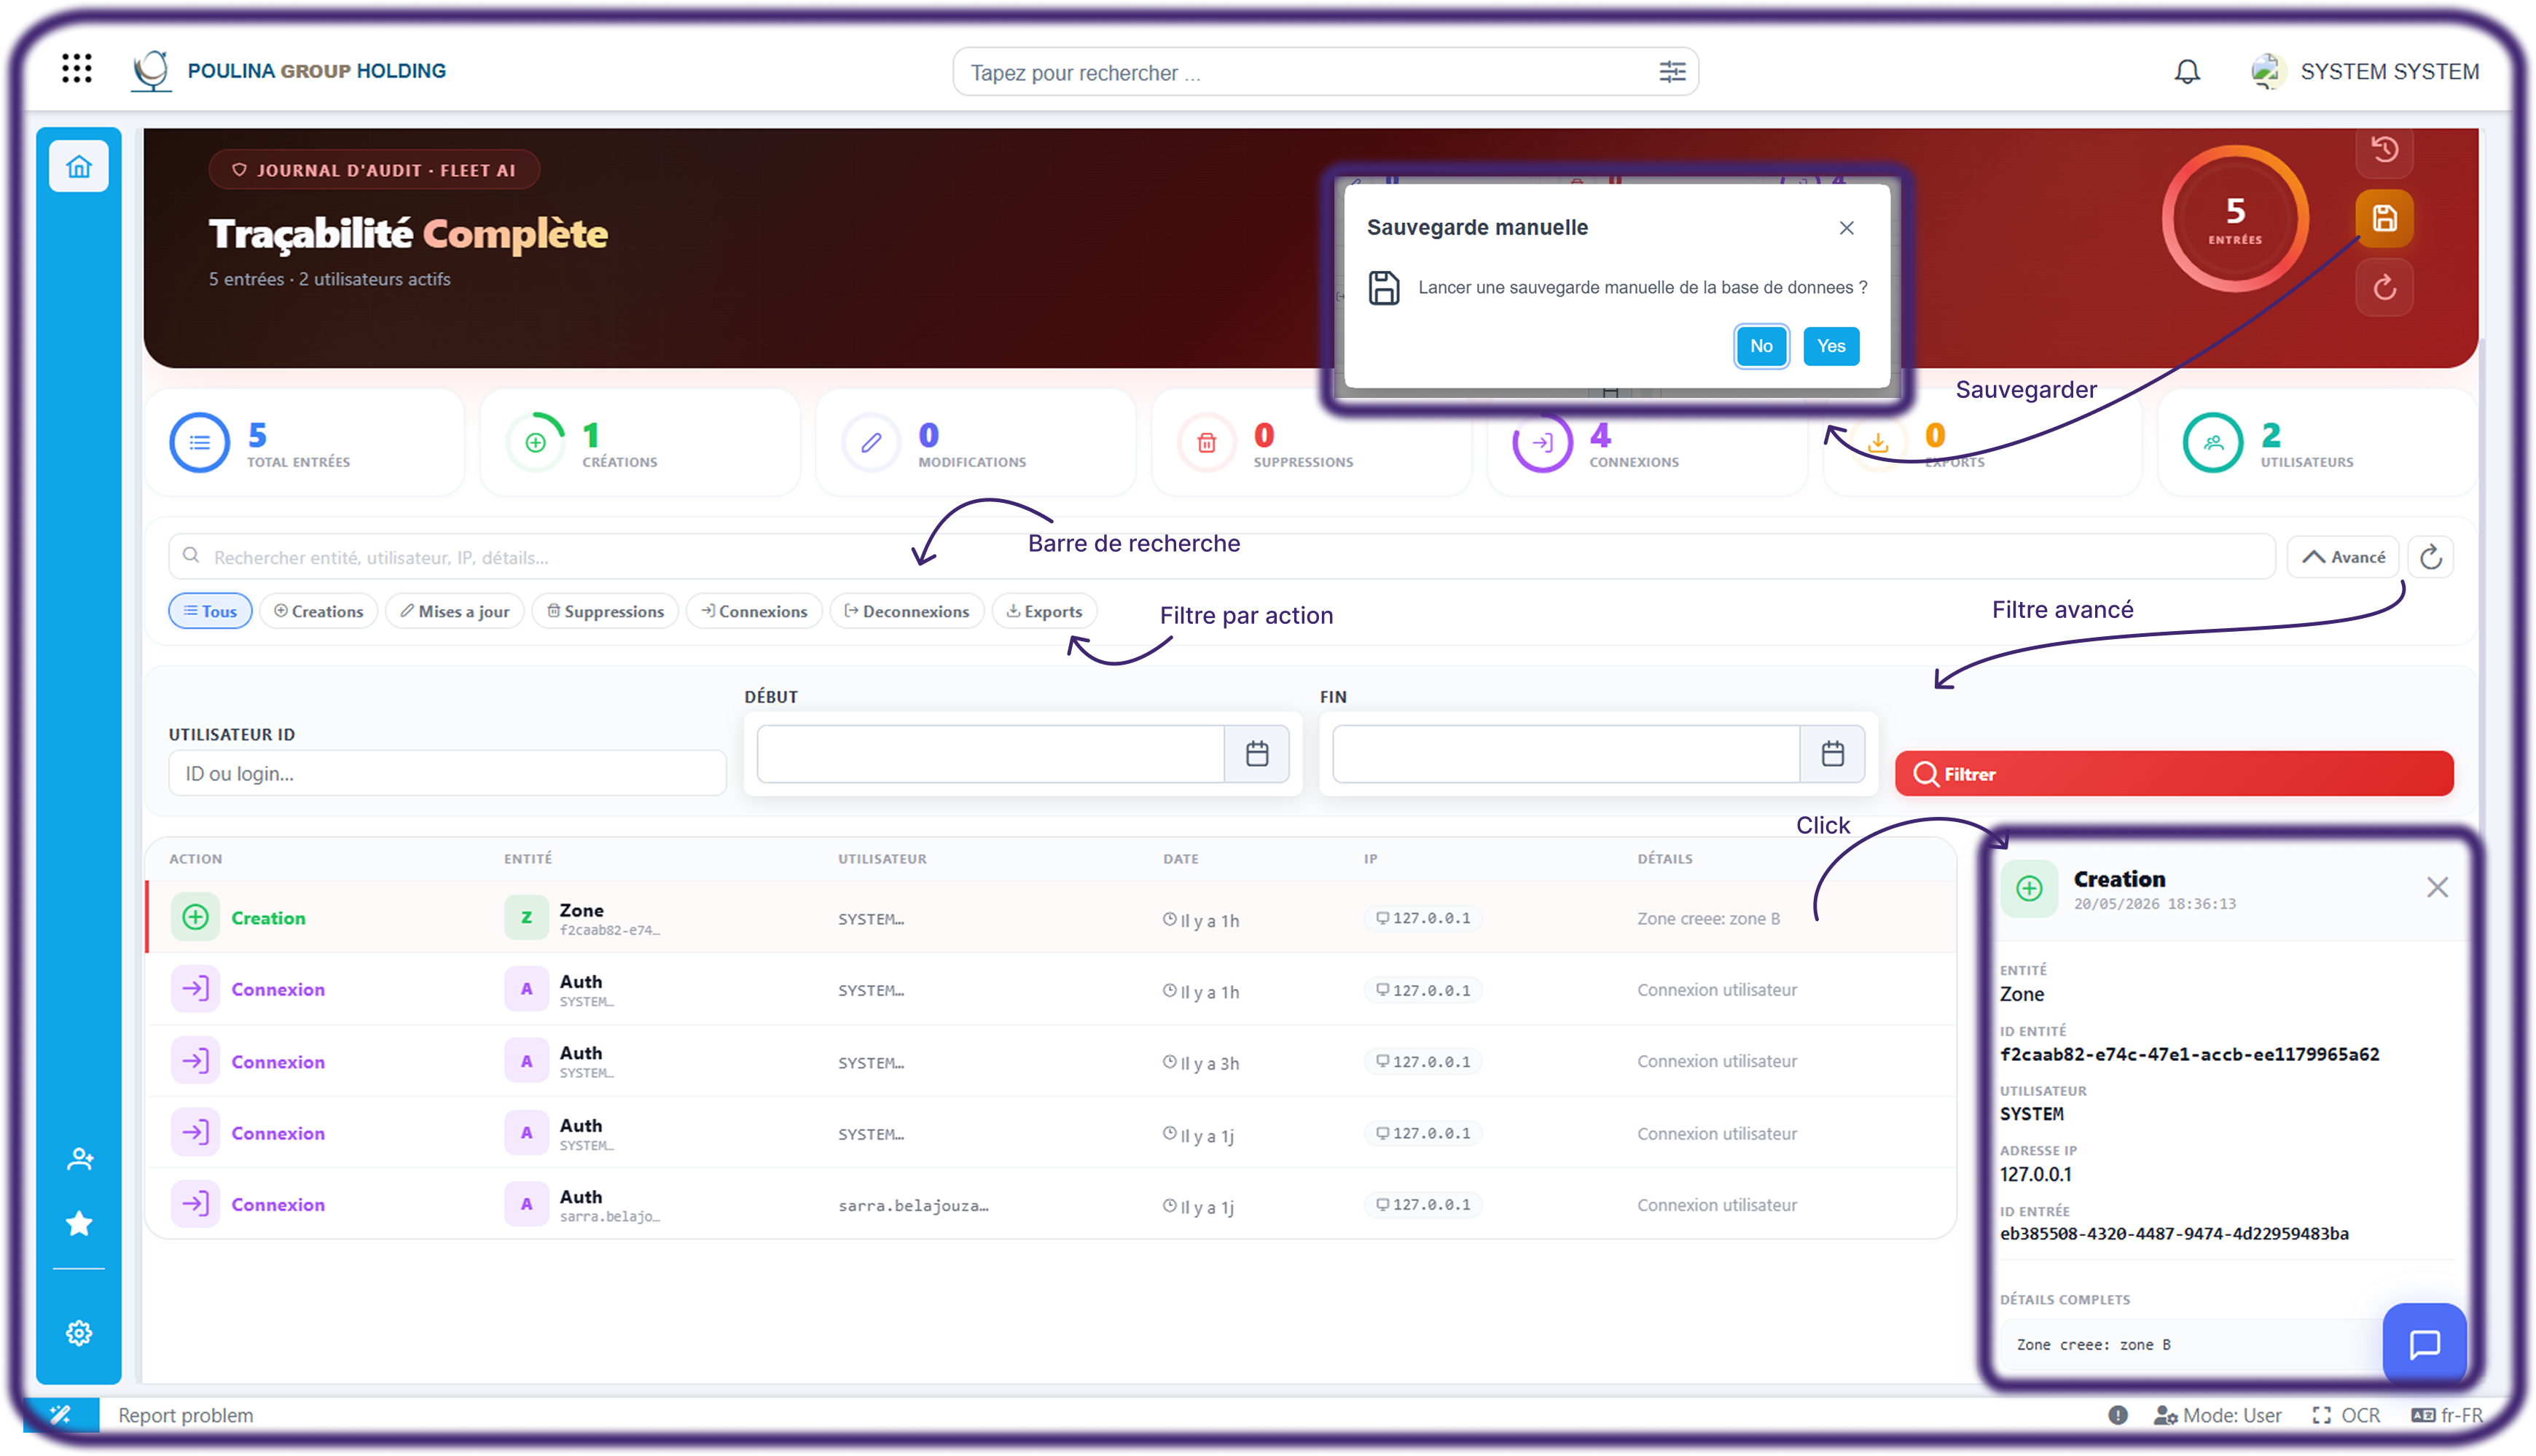
\includegraphics[width=\linewidth, keepaspectratio]{img/capture/web/sp1_audit_composite}%
}{%
  \fbox{\parbox{0.9\linewidth}{\centering\vspace{4cm}\textit{[img/sp1\_audit\_composite]}\vspace{4cm}}}%
}
\caption{Journal d'audit filtrable et déclenchement de sauvegarde}
\label{fig:sp1-audit}
\end{figure}

\subsection{Centre de notifications}

Le système intègre un centre de notifications temps réel (WebSocket). Les utilisateurs configurent leurs préférences (push in-app) par type d'événement.

\begin{figure}[H]
\centering
\IfFileExists{img/capture/web/sp1_notifications_composite.png}{%
  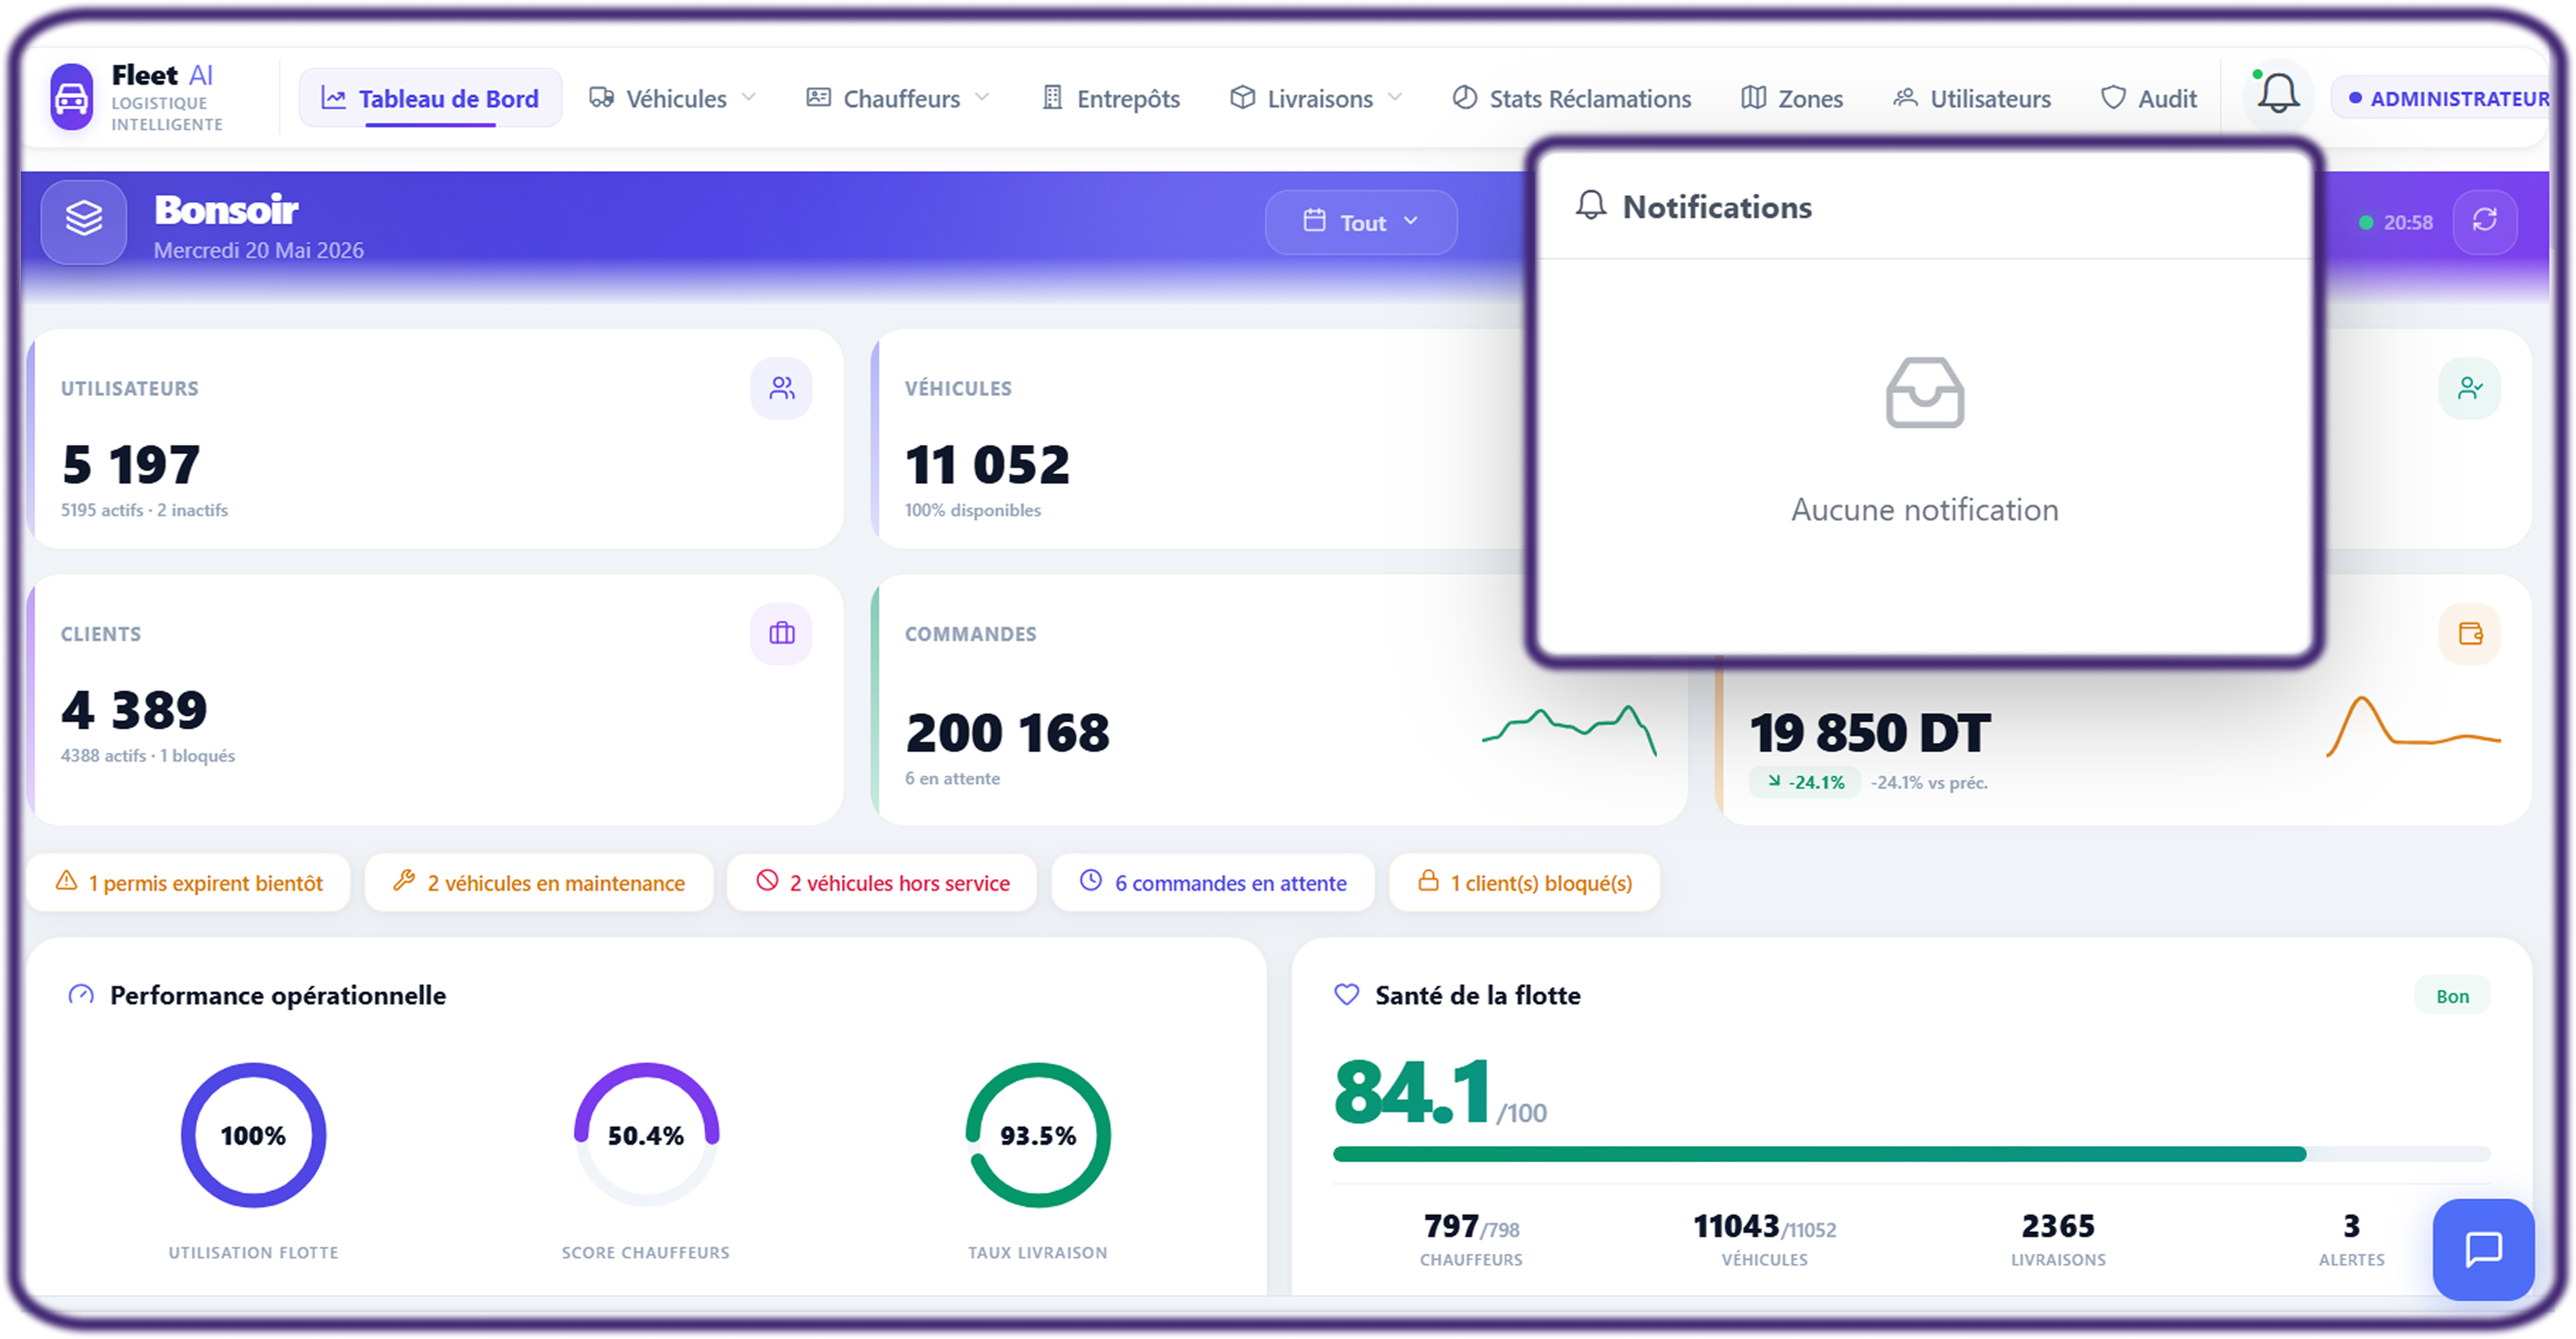
\includegraphics[width=\linewidth, keepaspectratio]{img/capture/web/sp1_notifications_composite}%
}{%
  \fbox{\parbox{0.9\linewidth}{\centering\vspace{4cm}\textit{[img/sp1\_notifications\_composite]}\vspace{4cm}}}%
}
\caption{Centre de notifications WebSocket et préférences}
\label{fig:sp1-notifications}
\end{figure}

% =============================================================
\section{Tests}
% =============================================================

Afin de garantir la fiabilité et la robustesse des fonctionnalités développées dès les fondations du projet, une validation rigoureuse a été mise en place à l'aide de tests unitaires.

\begin{itemize}
    \item \textbf{Les Tests Unitaires :} Ils permettent de valider le comportement précis d'un composant logiciel ou d'une méthode de manière totalement isolée, indépendamment du reste du système.
\end{itemize}

\begin{figure}[H]
\centering
\IfFileExists{img/capture/web/sp1_test_junit.png}{%
  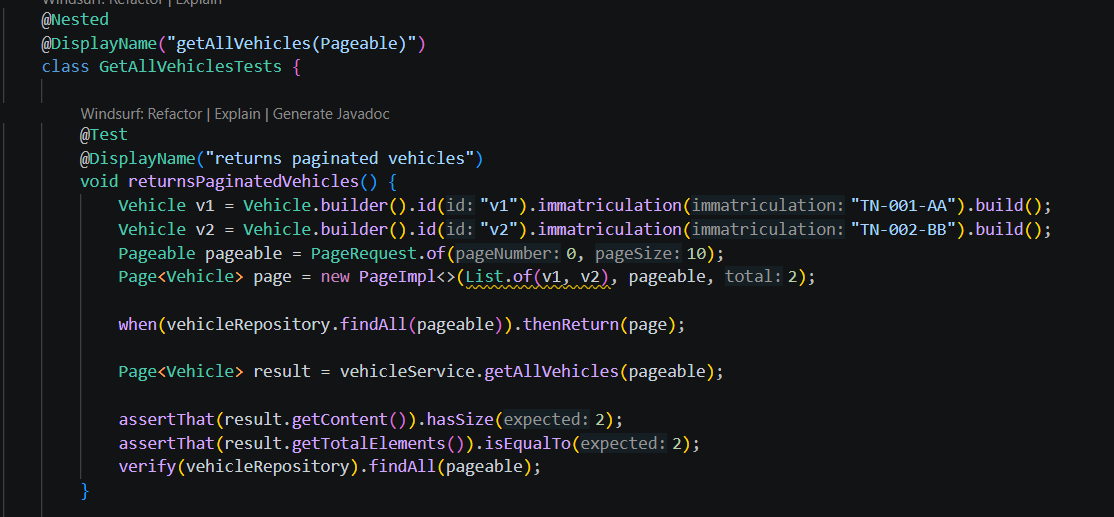
\includegraphics[width=\linewidth, keepaspectratio]{img/capture/web/sp1_test_junit}%
}{%
  \fbox{\parbox{0.9\linewidth}{\centering\vspace{4cm}\textit{[img/capture/web/sp1\_test\_junit.png]}\vspace{4cm}}}%
}
\caption{Exemple d'un test unitaire et résultat d'exécution (Succès)}
\label{fig:sp1-test}
\end{figure}

\section*{Conclusion}
\addcontentsline{toc}{section}{Conclusion}

Le Sprint~1 livre les fondations de Fleet~AI : authentification unifiée via la passerelle WFMS, contrôle d'accès par rôles, gestion complète des référentiels opérationnels (utilisateurs, véhicules, chauffeurs, zones) et journal d'audit avec double persistance. L'application mobile Flutter permet au Chauffeur de consulter son profil et ses performances. Ces composants constituent la base sur laquelle reposent tous les sprints suivants.
